\documentclass[withoutpreface,bwprint]{cumcmthesis}

%====================== 基本宏包 ======================
\usepackage{amsmath,amssymb,amsfonts}
\usepackage{geometry}
\usepackage{setspace}
\usepackage{graphicx}
\usepackage{float}
\usepackage{booktabs}
\usepackage{array}
\usepackage{longtable}
\usepackage{subcaption}
\usepackage{enumitem}
\usepackage{xcolor}
\usepackage{listings}
\hypersetup{hidelinks}

% 正文文献引用统一采用小号右上角方括号标注。
\makeatletter
\renewcommand{\@cite}[2]{\textsuperscript{\fontsize{7pt}{7pt}\selectfont[#1]}}
\makeatother

%====================== 页面设置 ======================
% 首先以零页边距嵌入官方承诺书，第二页起恢复竞赛规定页边距。
\geometry{a4paper,margin=0pt}
% 摘要首页严格按官方“承诺书和摘要页”中的附件2结构排版。
\newcommand{\makeofficialabstracthead}{%
  \thispagestyle{empty}%
  \noindent{\zihao{4}\songti 附件2：\par}
  \vspace{-0.6em}
  \begin{center}
    {\zihao{-2}\heiti\bfseries 2026年NUDT-CSU数学建模联赛\par}
    \vspace{0.5em}
    
\includegraphics[height=2.75cm]{figures/logo_nudt.png}%
    \hspace{0.35cm}%
    
\includegraphics[height=2.75cm]{figures/logo_csu.png}\par
  \end{center}
  \vspace{0.5em}
  \noindent\hspace{1.8cm}%
  {\zihao{4}\heiti\bfseries 题\quad 目：}%
  \begin{minipage}[t]{0.70\textwidth}
    \centering\zihao{4}\heiti\bfseries
    基于多尺度谱估计与鲁棒传感器融合的\\[-0.1em]
    机械设备故障检测研究
  \end{minipage}\par
  \vspace{0.7em}%
}

\renewenvironment{abstract}{%
  \begin{spacing}{1.5}%
  \setlength{\parindent}{2em}%
  \noindent{\zihao{-4}\songti\bfseries 摘\quad 要：}\par
  \vspace{0.5em}%
  \zihao{-4}\songti
}{%
  \end{spacing}%
}

\renewcommand{\keywords}[1]{%
  \par\vspace{0.6em}%
  {\zihao{-4}\heiti\noindent\bfseries 关键词：}%
  {\zihao{-4}\heiti\bfseries #1}%
}

% 摘要中的方法与结果使用黑体，确保中文在 PDF 中清晰加粗。
\newcommand{\absbold}[1]{{\heiti\bfseries #1}}

%====================== 代码格式 ======================
\lstset{
    basicstyle=\ttfamily\footnotesize,
    breaklines=true,
    frame=single,
    columns=fullflexible
}

\begin{document}
% 官方承诺书为论文第一页；身份信息栏保留待参赛队填写。
\thispagestyle{empty}
\vspace*{-\topskip}
\noindent\makebox[\paperwidth][c]{%
  \includegraphics[page=1,width=0.98\paperwidth,height=0.98\paperheight,keepaspectratio]{figures/official_commitment_source.pdf}%
}
\clearpage
\newgeometry{a4paper,left=31.8mm,right=31.8mm,top=25.4mm,bottom=25.4mm}
\makeofficialabstracthead
\begin{abstract}

机械设备早期微弱故障信号远弱于运行噪声，多源频率叠加与传感器受限增大识别难度。本文基于100Hz采样、400s振动时序数据，建立微弱故障检测、波形恢复、多源信号分离与传感器鲁棒布局递进模型。

\absbold{针对问题一：}单源弱故障检测需兼顾频谱分辨能力与估计稳定性。全段FFT频率分辨率更高，但单次周期图波动幅度较大；Welch分段平均谱能够降低噪声方差，却会损失部分分辨率。本文\absbold{结合两种谱估计方式构建联合检测模型，将单一谱分析改为双向互补校验，引入最大谱线检验控制全频段虚警概率}，\absbold{确定故障特征频率为2.0000Hz}。

\absbold{针对问题二：}已知故障频率后重构波形，直接对正弦信号开展非线性搜索易受初值、相位周期特性影响，极易出现局部收敛问题。本文\absbold{利用三角恒等变换将求解过程转化为线性最小二乘参数估计，通过正交基线性回归完成解析计算}，\absbold{得到故障振幅0.0352、初相1.574rad，残差均方根0.1000}；依托\absbold{残差重采样仿真}开展重复性测试，\absbold{波形归一化误差中位数为4.47\%}，验证波形恢复效果。

\absbold{针对问题三：}多故障源信号分离需要自动判断源数量，同时削弱不同分量之间的频谱干扰。阈值设置过严会遗漏幅值较弱的故障分量，逐一分量拟合则容易引发频谱泄漏。本文\absbold{依次完成候选频率筛选、借助BIC准则自动确定模型阶数、采用多频联合最小二乘实现信号拆分}，同步解决源数未知与参数耦合难题，\absbold{最终确定最优故障源数量为4，分离得到4.0000Hz、7.9999Hz、13.0001Hz、14.0000Hz四组故障分量}；通过\absbold{相邻双频分辨数值实验}证明，\absbold{该模型能够稳定区分间距0.005Hz及以上的邻近故障频率}。

\absbold{针对问题四：}传感器布设优化核心是在测点数量有限的前提下，提升所有故障源中最难检测分量的识别效果。综合振动传播衰减规律、测点空间噪声差异以及系统虚警率约束条件，\absbold{先计算单测点信噪比，再通过非相干能量融合整合多测点数据，搭建以max-min最差源检测概率为优化目标的鲁棒布局模型}。在典型算例中采用三点分散布设方案，\absbold{系统达到0.9检测概率的所需时长由单传感器220.7s缩短至64.4s}；利用\absbold{蒙特卡洛仿真校验}，\absbold{系统实际虚警率和预设0.01标准保持一致}。

最后，本文对整套模型进行综合评估：模型贴合工业设备监测实际工况，可有效解决微弱故障识别、多分量信号分离以及传感器优化布设相关问题，具备较强\absbold{实用性与计算效率}，同样能够应用于旋转机械故障诊断、结构健康监测、工业设备状态监测等相关领域。

\keywords{微弱故障检测；Welch谱估计；BIC模型选择；联合最小二乘；传感器鲁棒布局。}
\end{abstract}
\clearpage

% 目录部分使用大写罗马数字，从 I 开始编号。
\pagenumbering{Roman}
\setcounter{page}{1}
\pagestyle{plain}
\setlength{\cftsecnumwidth}{3.5em}
\tableofcontents
\clearpage

\begingroup
\setstretch{1.0}
\renewcommand{\cftfigpresnum}{图}
\setlength{\cftfignumwidth}{3em}
\renewcommand{\cfttabpresnum}{表}
\setlength{\cfttabnumwidth}{3em}
\listoffigures
\vspace{1em}
\listoftables
\endgroup
\clearpage

%====================== 正文 ======================
% 正文切换为阿拉伯数字，并从 1 重新编号。
\pagenumbering{arabic}
\setcounter{page}{1}
\pagestyle{plain}
\section{问题重述}

\subsection{问题背景}

旋转机械设备在长期运行中会因齿轮磨损、轴承裂纹、啮合冲击等原因产生周期性微弱振动，并已成为故障诊断研究的重要对象\cite{lv2022}。此类信号的能量通常远低于电机噪声、结构振动和测量噪声形成的背景基底，若仅在时域观察，早期故障特征会被完全淹没，导致传统阈值报警容易出现漏检或误报。

从信号处理角度看，故障分量虽弱，但是它的能量具有高度集中的频率结构，而噪声近似宽带分布。近年来，多变量信号处理也被用于复杂工况下的旋转机械故障诊断\cite{lv2022}。因而，若能在频域中提高谱估计分辨率并降低估计方差，就可以把“看不见”的时域周期在功率谱上显影。本文据此将故障检测建模为统计检测与参数估计问题，并进一步延伸到多源分离和传感器空间布局。

\subsection{问题提出}

题目给定的核心观测关系为：传感器采集信号 \(x(t)\) 由故障周期信号 \(s(t)\) 与背景噪声 \(n(t)\) 线性叠加而成。本文需要在单源和多源两类场景下完成频率检测、波形恢复、源数判定与传感器优化布局。具体任务可归纳为以下四个层次：

\begin{enumerate}[label=问题\arabic*：,leftmargin=4em]
    \item 在单源弱故障条件下，从强噪声时域序列中检测故障特征频率 \(f_0\)，并说明所用方法相对于传统傅里叶分析的优势。
    \item 在 \(f_0\) 已知基础上估计故障信号振幅 \(A\) 与初相 \(\varphi_0\)，恢复完整波形，并从时域和频域量化误差。
    \item 在故障源数量未知时，自动识别多个故障频率并估计各分量参数，同时讨论频率分辨极限。
    \item 基于设备几何结构和故障源位置，设计最多 \(3\) 个传感器的布局，使检测概率尽可能高、误报率尽可能低。
\end{enumerate}

\subsection{资料条件与本文工作}

附件提供单源与多源两组单通道时间序列，采样率 \(f_s=100\,\mathrm{Hz}\)，均含 \(N=40001\) 个采样点，对应观测时长 \(T=400\,\mathrm{s}\)。题目未给设备几何尺寸、故障源坐标、传播衰减系数及测点噪声场，因此问题四先建立不依赖具体几何的通用模型，再用明确标注的代表性场景说明求解流程。围绕这些数据，本文工作路线如图~\ref{fig:route} 所示。

\begin{figure}[H]
    \centering
    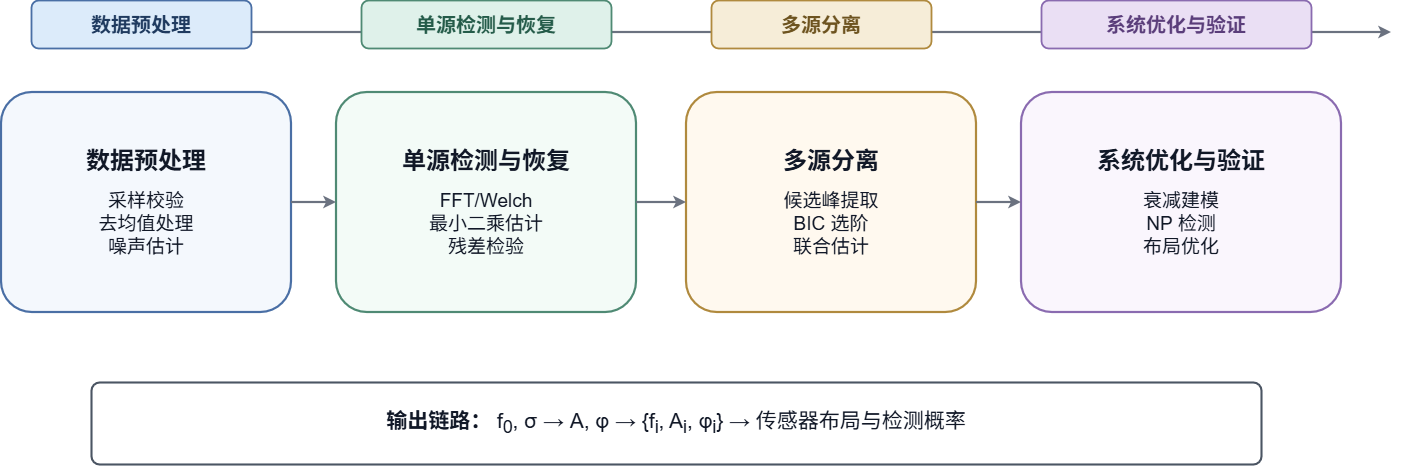
\includegraphics[width=0.98\textwidth]{技术路线图.png}
    \caption{总体技术路线}
    \label{fig:route}
\end{figure}

本文把四问组织成“前问输出作为后问输入”的闭环：问题一给出 \(f_0\) 与噪声基底，问题二给出单源振幅与相位，问题三给出多源数量、频率与振幅，问题四再将这些结果转化为传感器布局模型的输入。

\section{问题分析}

\subsection{问题一的分析}

单源检测的困难并不在于是否存在傅里叶峰值，而在于弱峰能否与随机噪声起伏可靠区分。FFT 可视为把时域序列投影到一组不同频率的复指数基上：周期故障分量在对应频率处相干叠加，宽带随机噪声则分散于各谱线。因此，全长序列可凭借较小的频率间隔 \(\Delta f=f_s/N\) 精确定位谱峰，但单次周期图的方差较大，噪声也可能形成偶然尖峰。Welch 方法将数据分成相互重叠的短段，对各段加 Hann 窗后分别计算周期图并取平均；加窗用于抑制有限截断引起的频谱泄漏，分段平均则抵消不同数据段中的随机起伏，以一定的频率分辨率损失换取更稳定的谱估计。

基于上述互补关系，本文采用“FFT 定位、Welch 复核、统计阈值判决”的联合流程：先利用全长 FFT 形成候选频率，再检查该峰是否在 Welch 平均谱中仍稳定存在，最后用 Bonferroni 校正控制遍历全频段带来的总体虚警率。这样既保留长序列的精细定位能力，又避免仅凭单次 FFT 最大峰作出判断；其改进并非提高 FFT 的理论分辨率，而是同时增强弱峰识别的稳定性并给出可量化的全频段误报约束。

\subsection{问题二的分析}

已知故障频率后，待求量仅为振幅与初相。若直接对正弦形式进行非线性搜索，结果会受到初值和相位周期性的影响。利用正弦、余弦两组正交基可把该问题改写成线性回归，再由两个回归系数还原振幅和相位。模型是否有效不能只看拟合曲线，还需比较残差均方根、频域峰值和参数区间，因此本文从时域与频域两方面进行误差检验。

\subsection{问题三的分析}

多源情形同时包含“源数未知”和“参数耦合”两类困难。阈值过严会遗漏弱分量，阈值过松又会引入噪声峰；逐个拟合还可能使相邻频率相互泄漏。本文先适度放宽寻峰条件形成候选集，再以信息准则在拟合误差与模型复杂度之间折中，确定源数后统一构建设计矩阵，使所有频率分量在同一次最小二乘计算中完成校正。本问所称“定位”是故障特征在频率轴上的定位；附件仅含单通道数据，缺少多测点传播信息，因而不能据此唯一确定故障源的物理空间位置。

\subsection{问题四的分析}

传感器布局既要靠近故障源以获得较强信号，也要避免多个测点集中在局部区域而造成覆盖失衡；相关研究表明，安装不确定性、测点聚集和优化目标选择都会影响布点质量\cite{an2022,hassani2023}。因为虚警率由报警制度预先约束，布局优劣可转化为固定系统总虚警率下检测概率的比较。本文用距离衰减描述传播损失，以噪声归一化的非相干能量融合汇总独立测点信息\cite{xiao2025}，并采用 max-min 准则优先改善最难检测的故障源，最终在可安装网格上搜索可执行方案\cite{deepseek2025}。

\section{模型假设}

为简化问题并保证模型具有明确的统计意义，本文作出如下假设：

\begin{enumerate}[label=假设\arabic*：,leftmargin=4em]
    \item \textbf{噪声局部平稳且条件高斯：}预处理后，背景噪声在分析窗内近似为零均值高斯弱平稳过程，目标频带内无无法辨别的强同频干扰。该条件为问题一的阈值、问题二和三的参数估计及问题四的卡方分布提供依据，并由残差正态性和自相关核验；若失配，则进行协方差预白化，并以稳健谱或残差 Bootstrap 标定阈值。
    \item \textbf{故障响应线性叠加：}在传感器线性工作区间内，观测量等于各故障周期分量与噪声之和。该条件支撑问题一至三的正交分解和最小二乘估计，也使问题四可分源计算信噪比；若残差存在显著谐波、调制边带或幅值相关结构，应增加非线性项或改用非线性系统辨识。
    \item \textbf{工况与参数窗内稳定：}设备在观测窗内近似恒速，各分量的频率、振幅和相位不发生突变，因而四问可使用定频正弦模型并传递参数；若转速或幅值明显漂移，应缩短分析窗，采用同步重采样、阶次谱或时变参数模型。
    \item \textbf{采样充分且时间基准准确：}采样间隔稳定，采样率满足奈奎斯特条件，\(0\sim20\,\mathrm{Hz}\) 频段不存在显著混叠。该条件保证问题一至三的频率轴、相位和分辨率有效；若欠采样或时钟失准，应先进行抗混叠采集、时间校准或重采样。
    \item \textbf{多测点噪声条件独立：}给定故障响应后，不同传感器噪声近似相互独立，使问题四可采用非相干能量融合并累加信噪比；若健康数据表明测点间显著相关，则估计完整噪声协方差矩阵，经空间预白化后重算联合统计量与阈值。
    \item \textbf{空间传播参数在检测期内稳定：}问题四中，各测点的传播增益和噪声尺度近似不变，距离衰减可作为缺少标定数据时的代理模型，使布局能统一比较；若存在反射、多路径或局部共振，应以试验频率响应 \(H_{ij}(f_j)\) 替代指数衰减关系。
\end{enumerate}

\textbf{算例条件说明：}问题四另取 \(4\,\mathrm{m}\times2\,\mathrm{m}\) 的代表性区域并按 \(0.25\,\mathrm{m}\) 离散。几何范围、网格、源位置和传播参数仅为可复现算例设置，并非题目事实或普遍假设；工程应用时须以真实图纸、可安装区域和现场标定结果替换后重新寻优。

\section{符号说明}

全文主要符号及单位见表~\ref{tab:symbols}，其余局部变量在首次出现时说明。

\begin{table}[H]
\centering
\small
\setlength{\tabcolsep}{4pt}
\renewcommand{\arraystretch}{1.08}
\caption{主要符号说明}
\label{tab:symbols}
\begin{tabular}{>{\centering\arraybackslash}m{3.2cm} m{7.5cm} >{\centering\arraybackslash}m{3cm}}
\toprule
符号 & 含义 & 单位/说明 \\
\midrule
\(x(t),x[k]\) & 传感器采集的连续/离散振动加速度信号 & a.u. \\
\(s(t)\) & 故障齿轮产生的弱周期信号 & — \\
\(n(t)\) & 背景噪声 & — \\
\(A,A_i\) & 单源/第 \(i\) 个故障分量振幅 & a.u. \\
\(f_0,f_i\) & 单源/第 \(i\) 个故障特征频率 & Hz \\
\(\varphi_0,\varphi_i\) & 单源/第 \(i\) 个故障分量初相 & rad \\
\(f_s,N,T\) & 采样率、采样点数、观测时长 & Hz、点、s \\
\(\Delta f\) & 频率分辨率，\(\Delta f=f_s/N\) & Hz \\
\(P_{\mathrm{FFT}},P_W\) & FFT 功率谱与 Welch 功率谱估计 & — \\
\(L,K,B\) & 分段长度、分段数、独立搜索频点数 & 点、段、个 \\
\(M\) & 故障源数量 & 个 \\
\(\mathrm{BIC}\) & 贝叶斯信息准则，用于模型阶数选择 & — \\
\(d_{ij}\) & 第 \(i\) 个传感器到第 \(j\) 个故障源的距离 & m \\
\(\alpha\) & 信号传播的指数衰减系数 & \(\mathrm{m}^{-1}\) \\
\(\rho_{ij},\rho^{(j)}_{\mathrm{eq}}\) & 单传感器/融合等效信噪比 & — \\
\(P_{FA}^{\mathrm{sys}},P_{FA}^{(1)},P_D\) & 系统总虚警率、单频虚警率、检测概率 & — \\
\(g_{ij},\sigma_i\) & 测点灵敏度系数、位置相关噪声标准差 & — \\
\(N_o,q\) & 检测窗样本数、选用传感器数 & 点、个 \\
\(\lambda_j,\gamma_q\) & 非中心参数、检测阈值 & — \\
\(\Omega,\mathcal S\) & 候选安装点集合、所选传感器集合 & — \\
\(RSS_M,k_M\) & \(M\) 阶模型残差平方和、参数个数 & — \\
\bottomrule
\end{tabular}
\end{table}

\section{数据预处理}

\subsection{时域信号核验}

首先读取附件中的时间序列，按表~\ref{tab:preprocess} 核验采样间隔并去均值。单源数据均值为 \(4.467\times10^{-5}\)，标准差为 \(0.103063\)；多源数据标准差为 \(0.106421\)。两表均有 \(40001\) 个样本，时间从 \(0\) 到 \(400\,\mathrm{s}\)，不存在把“样本点数”误写成“采样区间数”的问题。

\begin{table}[H]
\centering
\small
\setlength{\tabcolsep}{3pt}
\renewcommand{\arraystretch}{1.05}
\caption{时域数据预处理流程}
\label{tab:preprocess}
\begin{tabular}{>{\centering\arraybackslash}m{2.5cm} m{6.1cm} m{5.1cm}}
\toprule
项目 & 处理方式 & 目的 \\
\midrule
采样率核验 & 由相邻时间戳差分估计 \(f_s=100\,\mathrm{Hz}\) & 确认频率轴与奈奎斯特条件 \\
去均值 & \(x[k]\leftarrow x[k]-\mathrm{mean}(x)\) & 削弱直流峰对谱估计的影响 \\
异常检查 & 检查缺失、重复与极端跳点 & 保证 FFT/Welch 不受非物理点污染 \\
短时可视化 & 绘制前 \(5\,\mathrm{s}\) 时域波形 & 说明时域弱故障不可直接辨识 \\
\bottomrule
\end{tabular}
\end{table}

\subsection{频域数据规约}

频域处理的关键是根据问题目标选择合适的谱估计尺度\cite{proakis2006,bendat2010}。单段全信号 FFT 保留最高频率分辨率，适合精确定位单频谱峰；Welch 方法通过分段加窗平均降低谱估计方差，适合验证峰值稳健性。本文将两者配合使用，避免“单次 FFT 偶然峰值”与“短窗频率分辨率不足”两个常见问题。

\subsection{空间几何数据构造}

题目没有给出可直接计算坐标的设备图纸。为展示通用模型的数值求解，本文另设代表性矩形区域 \([0,4]\times[0,2]\)，将四个源放在 \((0.5,1.0)\)、\((1.5,0.3)\)、\((2.5,1.7)\)、\((3.5,1.0)\)。仅取边界内侧的 \(0.25\,\mathrm{m}\) 网格，得到 \(105\) 个候选点；三传感器组合数为
\[
    C(105,3)=187460,
\]
规模适中，可直接穷举获得该代表性场景下的离散全局最优解。源坐标、区域尺寸、衰减系数和噪声场均属于算例设定，不当作题设条件。

\section{模型建立}

\subsection{问题一：单源故障频率检测模型}

问题一是在强噪声下进行单频率统计检测。离散观测模型为：
\begin{equation}
    x[k]=A\sin(2\pi f_0 k\Delta t+\varphi_0)+n[k],
    \quad k=0,1,\ldots,N-1 .
    \label{eq:obs}
\end{equation}

对 \(x[k]\) 作离散傅里叶变换，得到频域表示：
\begin{equation}
    X[m]=\sum_{k=0}^{N-1}x[k]e^{-j2\pi mk/N},
    \quad f_m=m\frac{f_s}{N}.
    \label{eq:dft}
\end{equation}

定义归一化单边功率谱：
\begin{equation}
    P_{\mathrm{FFT}}[m]=\left|\frac{X[m]}{N}\right|^2,
    \quad 0\leq m\leq \left\lfloor\frac{N}{2}\right\rfloor .
    \label{eq:psd}
\end{equation}

当信号中存在振幅为 \(A\) 的纯正弦分量时，其能量集中在 \(f_0\) 附近，而噪声能量分散在频率轴上，因此谱峰与噪声基底的理论比值近似为：
\begin{equation}
    \mathrm{SNR}_{\mathrm{spec}}
    \approx
    \frac{(A/2)^2}{\sigma_n^2/N}
    =
    \frac{NA^2}{4\sigma_n^2}.
    \label{eq:snrspec}
\end{equation}

式~\eqref{eq:snrspec} 直接解释了长时间采样对弱信号检测的优势：\(N\) 越大，单频信号在频域累积得越突出。为降低单段 FFT 的随机波动，本文进一步采用 Welch 分段平均谱\cite{welch1967}：
\begin{equation}
    P_W(f)=
    \frac{1}{K}
    \sum_{i=1}^{K}
    \frac{1}{f_s W_{ss}}
    \left|
    \sum_{l=0}^{L-1}x_i[l]w[l]e^{-j2\pi fl/f_s}
    \right|^2 .
    \label{eq:welch}
\end{equation}

其中，\(L\) 为每段样本数，\(K\) 为参与平均的分段数，\(w[l]\) 为 Hann 窗，\(W_{ss}=\sum_{l=0}^{L-1}w^2[l]\) 用于校正窗函数造成的能量尺度变化。若各段周期图近似独立，同一频点的平均可显著减小估计方差；采用 50\% 重叠则能在加窗后提高数据利用率。由于分段使频率间隔由 \(f_s/N\) 增至 \(f_s/L\)，故 Welch 谱仅承担稳健性复核，全长 FFT 仍用于报告最终频率。

最终故障频率估计为功率谱达到最大值的位置：
\begin{equation}
    \hat f_0=
    \mathop{\arg\max}_{f\in(0,f_s/2)}P(f),
    \quad
    P\in\{P_{\mathrm{FFT}},P_W\}.
    \label{eq:f0est}
\end{equation}

为控制在 \(0\sim20\,\mathrm{Hz}\) 全频带搜索造成的多重比较效应，本文以最大谱线而非单个预定频点构造检验。将系统允许的总虚警率记为 \(P_{FA}\)，Bonferroni 校正把每条谱线的显著性水平分配为 \(\alpha=P_{FA}/B\)。白噪声条件下，以噪声均值归一化的单频点周期图近似服从单位均值指数分布，故 \(\Pr\{Y>\eta\}=e^{-\eta}\)，从而得到阈值
\begin{equation}
 \eta=-\ln\!\left(\frac{P_{FA}}{B}\right).
 \label{eq:global-threshold}
\end{equation}
由并集上界可知，\(\Pr\{\max_bY_b>\eta\}\leq B\alpha=P_{FA}\)，因此该校正不要求各谱线严格独立，且比逐频点判断更能避免“搜索频点越多、偶然峰越多”的问题。本题在 \(0\sim20\,\mathrm{Hz}\) 内搜索 \(B=8000\) 个正频率谱线，取总虚警率 \(P_{FA}=0.01\) 时阈值约为噪声均值的 \(13.59\) 倍，而观测峰值比约为 \(1072\)，故结论不依赖主观画线。该阈值仍依赖单频点指数分布近似；若残差呈显著有色特征，应改用预白化或残差 Bootstrap。Welch 采用 Hann 窗、\(L=8192\)、50\% 重叠，频率分辨率为 \(0.012207\,\mathrm{Hz}\)，用于稳健复核而非替代全长 FFT 的精定位。

本模型输出单源特征频率及噪声基底，前者直接进入问题二的谐波参数估计，二者共同为后续检测阈值和仿真噪声尺度提供依据。

\subsection{问题二：单源故障波形恢复模型}

在问题一得到 \(f_0\) 后，正弦信号的未知参数只剩振幅和相位。利用三角恒等式将非线性参数估计转化为线性回归：
\begin{equation}
    s(t)=A\sin(2\pi f_0t+\varphi_0)
    =c_s\sin(2\pi f_0t)+c_c\cos(2\pi f_0t),
    \label{eq:linreg}
\end{equation}
其中
\[
    c_s=A\cos\varphi_0,\quad
    c_c=A\sin\varphi_0 .
\]

对所有采样点构造设计矩阵：
\begin{equation}
    \Phi=
    \begin{bmatrix}
    \sin(2\pi f_0 t_1) & \cos(2\pi f_0 t_1)\\
    \vdots & \vdots\\
    \sin(2\pi f_0 t_N) & \cos(2\pi f_0 t_N)
    \end{bmatrix},
    \quad
    \theta=
    \begin{bmatrix}
    c_s\\
    c_c
    \end{bmatrix}.
    \label{eq:design}
\end{equation}

最小二乘估计解析解为\cite{kay1993}：
\begin{equation}
    \hat{\theta}
    =
    (\Phi^T\Phi)^{-1}\Phi^T x .
    \label{eq:ls}
\end{equation}

由 \(\hat c_s\)、\(\hat c_c\) 还原振幅与初相：
\begin{equation}
    \hat A=\sqrt{\hat c_s^2+\hat c_c^2},
    \quad
    \hat{\varphi}_0=\operatorname{atan2}(\hat c_c,\hat c_s).
    \label{eq:amp}
\end{equation}

由于附件未提供无噪声真值，本文不能直接计算 \(\hat s\) 与真实 \(s\) 的恢复误差，而以残差均方根和分段参数稳定性作为间接评价，并用已知真值的残差重采样仿真检验恢复算法本身。残差均方根为
\begin{equation}
    \mathrm{RMSE}=
    \sqrt{
    \frac{1}{N}
    \sum_{k=1}^{N}
    \left(x[k]-\hat{s}[k]\right)^2
    }.
    \label{eq:rmse}
\end{equation}

本模型输出单源振幅、初相及恢复波形，并通过附件残差检验和有真值仿真分别评价数据拟合质量与算法恢复误差。

\subsection{问题三：多故障源自动分离模型}

多源场景下信号可表示为多个弱周期分量叠加：
\begin{equation}
    x(t)=
    \sum_{i=1}^{M}A_i\sin(2\pi f_i t+\varphi_i)+n(t).
    \label{eq:multi}
\end{equation}

由于 \(M\) 未知，本文先通过宽松阈值从 FFT 功率谱中提取候选峰，再对不同阶数 \(M\) 构造联合最小二乘模型，利用 \(\mathrm{BIC}\) 抑制过拟合\cite{schwarz1978}：
\begin{equation}
    \mathrm{BIC}(M)=
    N\ln\left(\frac{RSS_M}{N}\right)+k_M\ln N .
    \label{eq:bic}
\end{equation}

其中 \(k_M\) 为参数个数。虽然候选峰在选阶阶段暂时固定，但频率由同一数据筛选，仍会消耗模型自由度，为避免低估复杂度，本文保守取 \(k_M=3M\)，分别对应频率、正弦系数和余弦系数。确定 \(M^*\) 后，再连续优化频率并联合更新全部参数。

多频率联合最小二乘模型为：
\begin{equation}
    x(t)=
    \sum_{i=1}^{M}
    \left[
    \alpha_i\sin(2\pi f_i t)+
    \beta_i\cos(2\pi f_i t)
    \right]
    +n(t).
    \label{eq:jointls}
\end{equation}

本模型输出周期分量数及各分量的频率、振幅和初相，为问题四的多频率检测器、源强输入和最弱源鲁棒准则提供参数。

\subsection{问题四：传感器融合检测与布局优化模型}

问题四需要把信号估计结果转化为空间布设方案。设第 \(i\) 个传感器到第 \(j\) 个故障源的距离为 \(d_{ij}\)，\(g_{ij}\) 表示传播路径和安装方式造成的灵敏度差异，接收振幅为
\begin{equation}
    A_{ij}=A_jg_{ij}\exp(-\alpha d_{ij}),
    \label{eq:decay}
\end{equation}
其中 \(A_j\) 直接采用问题三估计的各源振幅。允许噪声随测点变化，单样本信噪比为
\begin{equation}
    \rho_{ij}=
    \frac{A_{ij}^2}{2\sigma_i^2}.
    \label{eq:rho}
\end{equation}
对每个已知故障频率，用正、余弦两个正交分量构造非相干能量统计量。选择 \(q\) 个传感器、每个检测窗含 \(N_o\) 个样本时，零假设和备择假设下分别有
\begin{equation}
 Z_j\mid H_0\sim\chi^2_{2q},\qquad
 Z_j\mid H_1\sim\chi'^2_{2q}(\lambda_j),qquad
 \lambda_j=N_o\sum_{i\in\mathcal S}\rho_{ij}.
 \label{eq:dist}
\end{equation}
同时监测 \(J=4\) 个故障频率时，先给定系统总虚警率 \(P_{FA}^{\mathrm{sys}}\)。为避免依赖不同频率统计量相互独立这一理想条件，本文采用 Bonferroni 分配
\begin{equation}
 P_{FA}^{(1)}=\frac{P_{FA}^{\mathrm{sys}}}{J},\qquad
 P\!\left(\bigcup_{j=1}^{J}\{Z_j>\gamma_q\}\middle|H_0\right)
 \leq\sum_{j=1}^{J}P_{FA}^{(1)}=P_{FA}^{\mathrm{sys}}.
 \label{eq:bonferroni}
\end{equation}
因此单频阈值与检测概率为
\begin{equation}
    \gamma_q=F_{\chi^2_{2q}}^{-1}\!\left(1-P_{FA}^{(1)}\right),\qquad
    P_D^{(j)}=1-F_{\chi'^2_{2q}(\lambda_j)}(\gamma_q).
    \label{eq:threshold}
\end{equation}
该统计量是噪声归一化的非相干能量融合，而非需要已知跨测点相位的相干最大比合并。独立传感器的信息贡献按信噪比相加：
\begin{equation}
    \rho_{\mathrm{eq}}^{(j)}
    =
    \sum_{i\in\mathcal S}\rho_{ij}.
    \label{eq:mrc}
\end{equation}
在候选安装点集合 \(\Omega\) 上，最多三个传感器的鲁棒布局模型为
\begin{equation}
    \max_{\mathcal S\subseteq\Omega,\,1\leq|\mathcal S|\leq3}
    \min_j P_D^{(j)}(\mathcal S).
    \label{eq:maxmin}
\end{equation}
题目要求兼顾检测与误报。本文采用 Neyman--Pearson 固定虚警率思想\cite{neyman1933}：先约束系统总 \(P_{FA}^{\mathrm{sys}}\)，再最大化最差源的 \(P_D\)。由于未知相位使备择假设成为复合假设，本文不宣称该能量统计量在所有检验中一致最优。因题目没有说明四个频率与空间源位置的一一对应关系，算例按问题三最弱振幅、\(\alpha=0.8\)、噪声尺度1.2及 \(g_{ij}=0.85\) 的不利组合进行保守设计，再在名义参数和扰动参数下评估同一布局。

本模型输出不超过三个测点的区域级布局及其检测概率、虚警率和报警时间；获得真实图纸与标定数据后，只需替换传播矩阵和噪声协方差即可重新求得安装坐标。

\section{模型结果与分析}

\subsection{问题一结果：单源频率检测}

FFT 精细谱定位得到故障峰
\[
    \hat f_0=2.0000\,\mathrm{Hz},
\]
谱峰与噪声中位基底之比约为 \(1782\)；Welch 估计在 \(f\approx2.0020\,\mathrm{Hz}\) 处给出一致峰值，差异仅为一个 Welch 频率分辨单元量级。如图~\ref{fig:q1time} 所示，时域波形难以直接辨识周期性，而两种频谱均在2 Hz附近形成稳定峰值。

\begin{figure}[H]
    \centering
    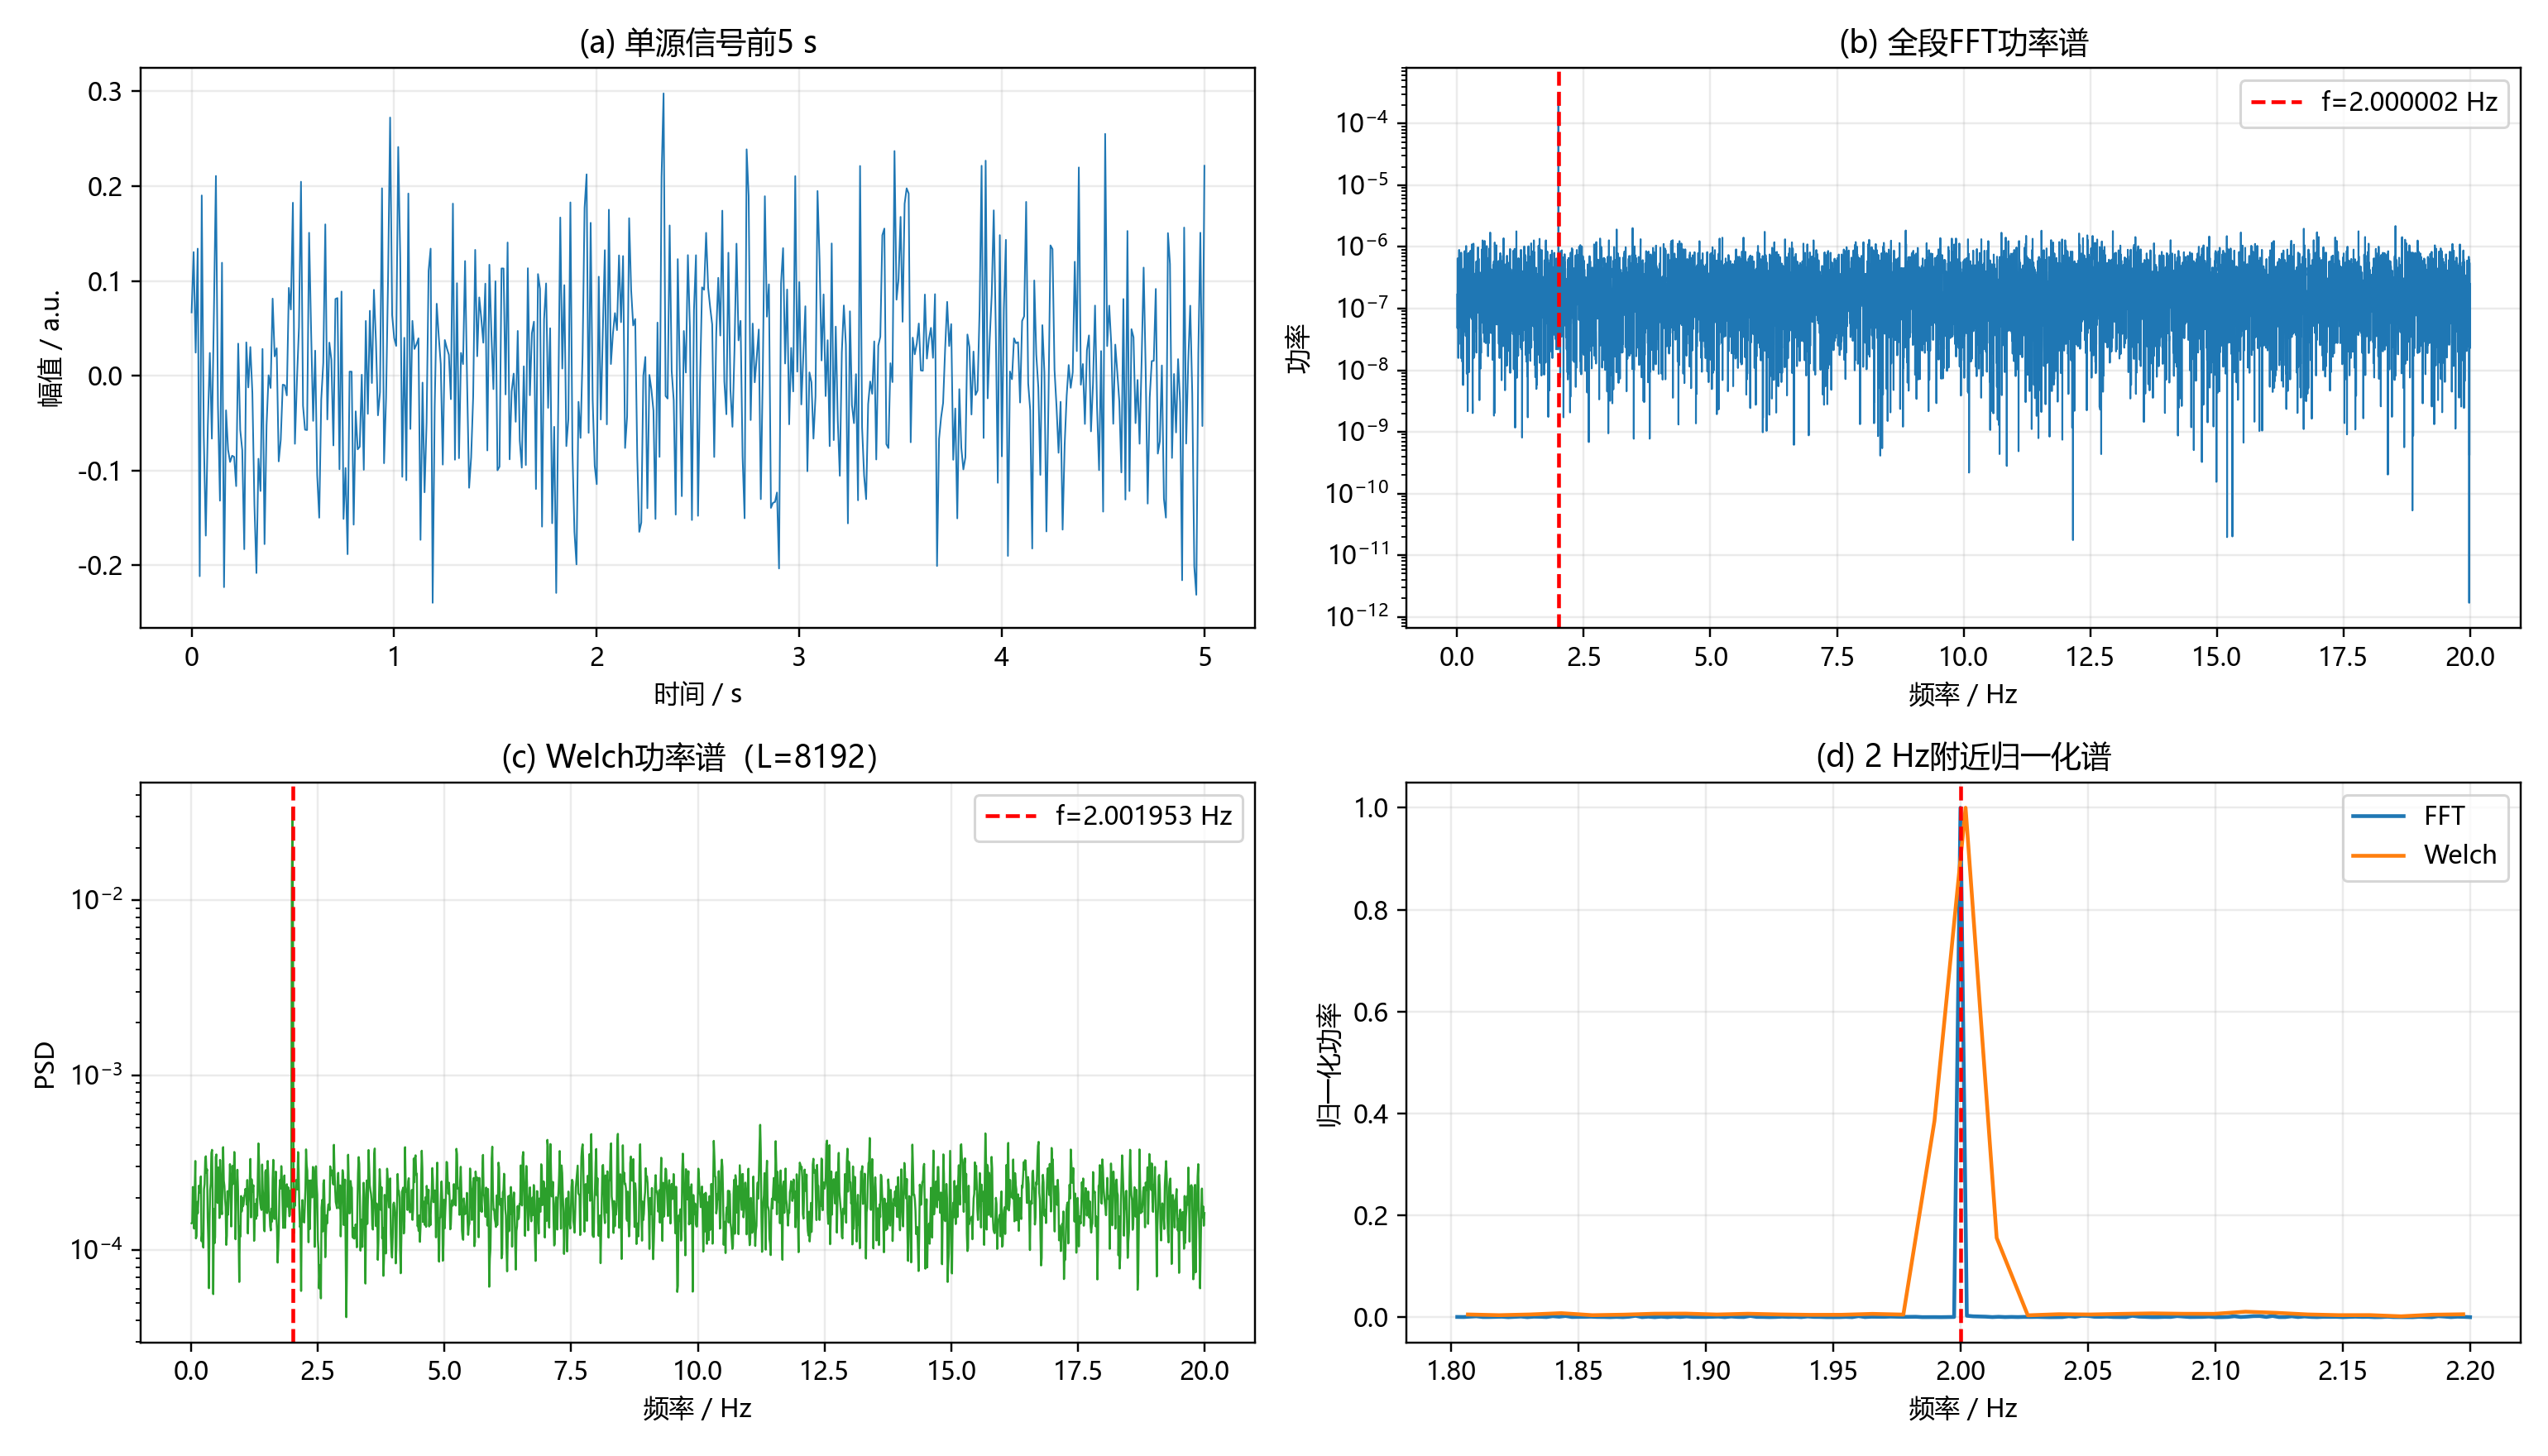
\includegraphics[width=0.90\textwidth,height=0.60\textheight,keepaspectratio]{figures/图1.png}
    \caption{单源故障信号时频分析}
    \label{fig:q1time}
\end{figure}

\begin{table}[H]
\centering
\small
\setlength{\tabcolsep}{2pt}
\renewcommand{\arraystretch}{1.2}
\caption{三种频谱分析方法定量对比}
\label{tab:methods}
\begin{tabular}{>{\centering\arraybackslash}m{2.0cm} >{\centering\arraybackslash}m{2.2cm} >{\centering\arraybackslash}m{1.2cm} >{\centering\arraybackslash}m{2.4cm} >{\centering\arraybackslash}m{1.8cm} >{\centering\arraybackslash}m{2.0cm}}
\toprule
分析方法 & \(\Delta f/\mathrm{Hz}\) & 分段数 & 峰值/谱中位基底 & 噪声基底CV & 全频带虚警控制 \\
\midrule
STFT \(L=256\) & 0.390625 & 311 & 6.21 & -- & 否 \\
全段FFT \(L=N\) & 0.002500 & 1 & 1782.04 & 1.004 & 否 \\
Welch \(L=8192\) & 0.012207 & 8 & 176.66 & 0.361 & 联合检验后是 \\
\bottomrule
\end{tabular}
\end{table}

\begin{figure}[H]
    \centering
    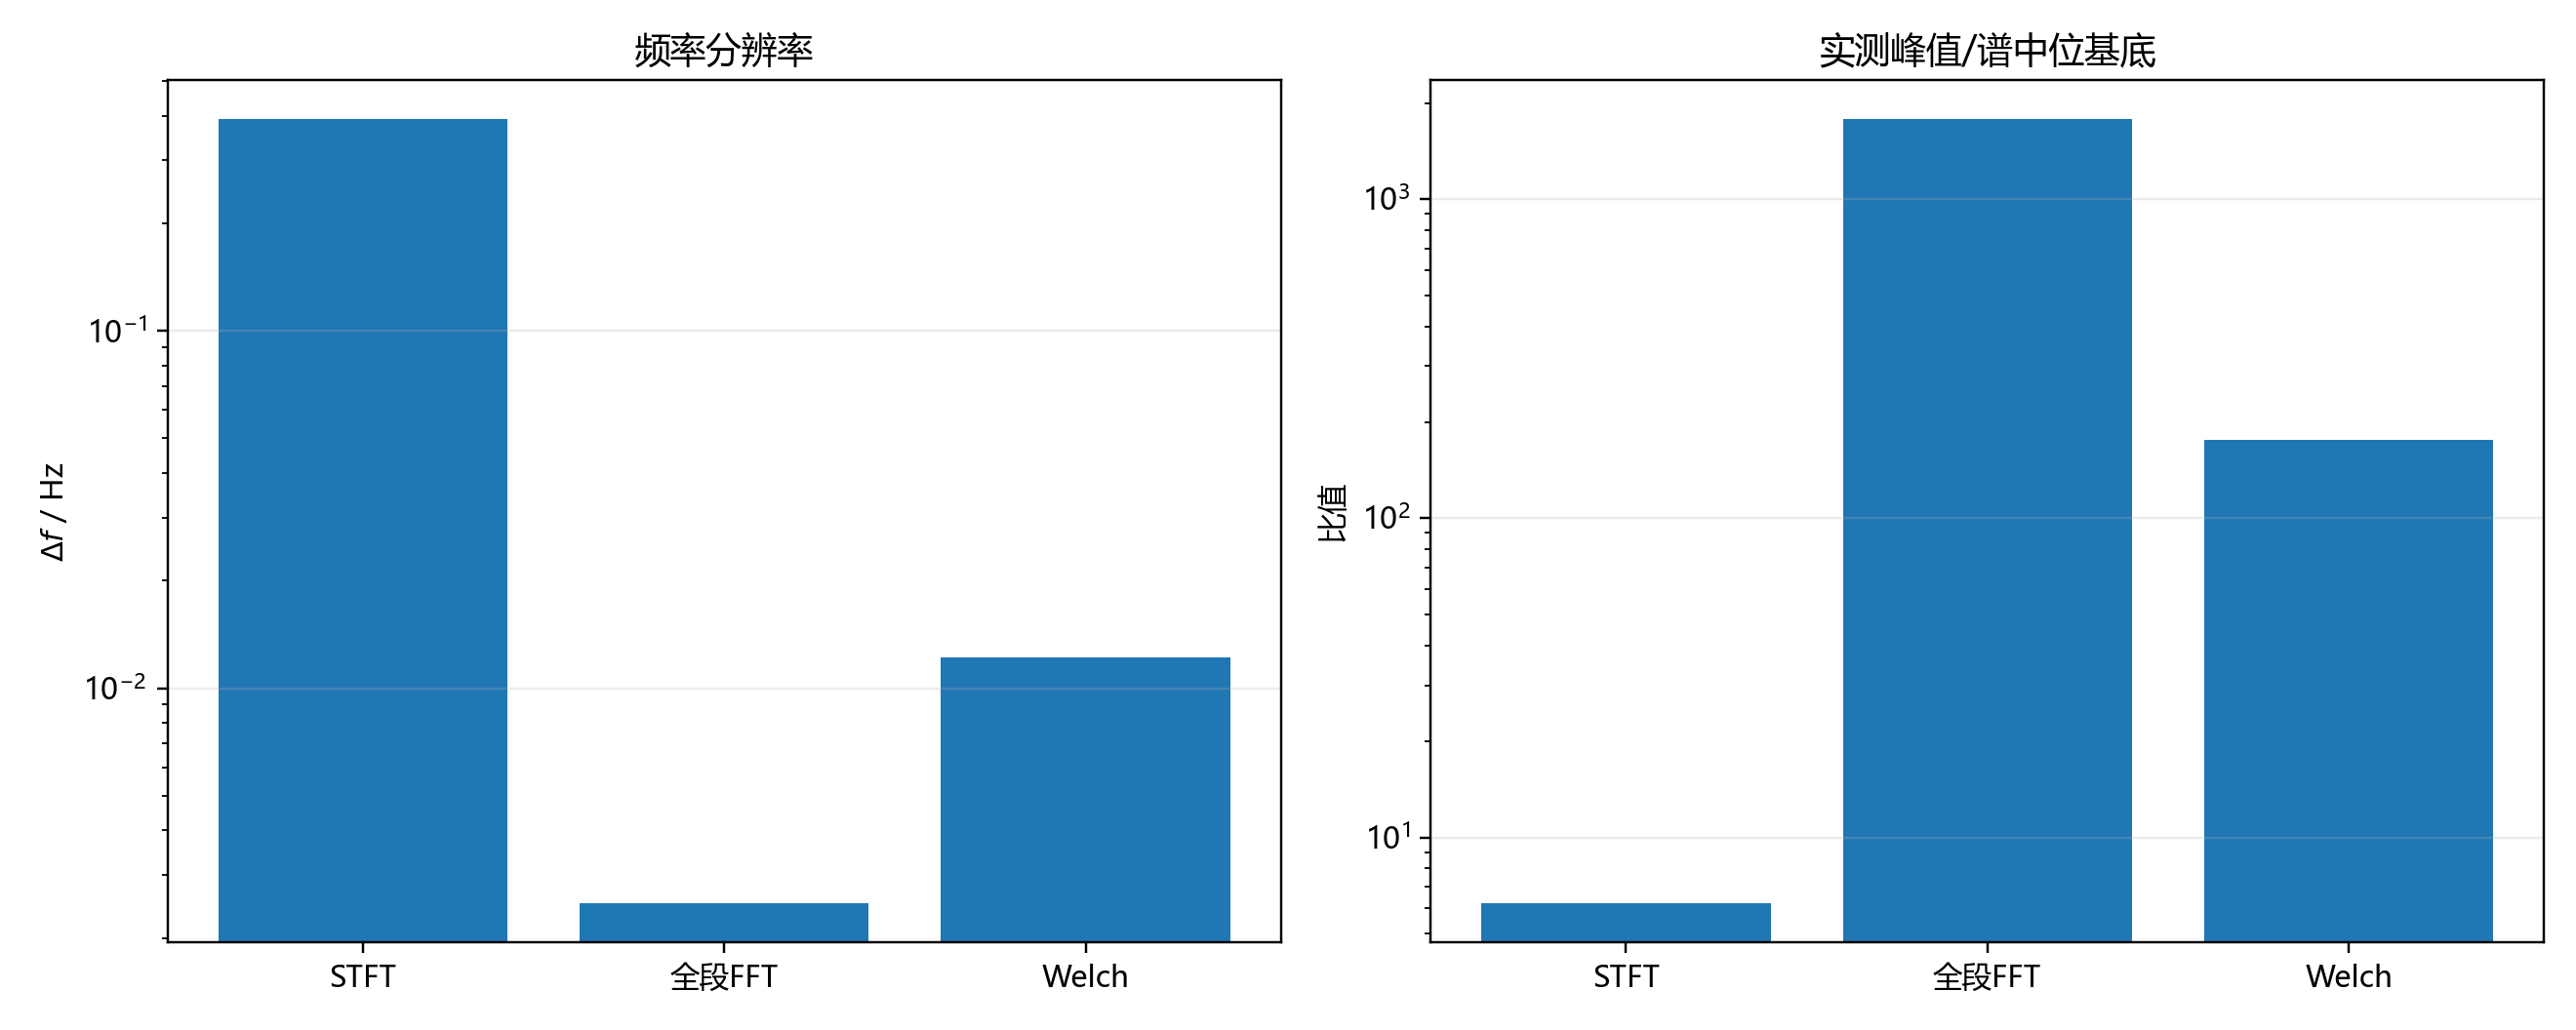
\includegraphics[width=0.88\textwidth,height=0.55\textheight,keepaspectratio]{figures/图2.png}
    \caption{频谱分析方法性能对比}
    \label{fig:q1compare}
\end{figure}

图~\ref{fig:q1compare} 与表~\ref{tab:methods} 均直接由附件数据计算，不再混用不同自由度下的理论检测概率。STFT保留时间定位能力但频率分辨率最低；全段FFT适合精确定位但单次周期图波动较大；Welch把噪声谱基底离散系数由1.004降至0.361，降低约64.1\%，且八个输入分段均在2 Hz附近检出主峰。因而本文以全段FFT定位、Welch复核，再联合最大谱线检验控制全频带虚警；相较只查看传统FFT谱峰，该流程同时给出跨时段稳定性和统计显著性证据。

\subsection{问题二结果：波形恢复与误差评价}

连续频率精化与最小二乘联合求解得到
\[
    \hat{A}=0.0352,\quad
    \hat{\varphi}_0=1.574\,\mathrm{rad}.
\]
恢复信号为：
\begin{equation}
    \hat{s}(t)=0.0352\sin(2\pi\times2.0000t+1.574).
    \label{eq:recovery}
\end{equation}

残差 \(\mathrm{RMSE}=0.1000\)，最大1--20阶绝对自相关为0.0094，Jarque--Bera检验 \(p=0.669\)，支持高斯白噪声近似。分别使用前、后200 s数据估计得到振幅0.03585和0.03453，相差3.7\%，说明周期参数在观测期内稳定。由于真实无噪声波形未知，以上指标评价的是模型残差和参数稳定性，不能解释为 \(\hat s\) 对真实 \(s\) 的直接RMSE。如图~\ref{fig:q2recovery} 所示，恢复分量具有稳定周期，残差未保留明显同频结构。

\begin{figure}[H]
    \centering
    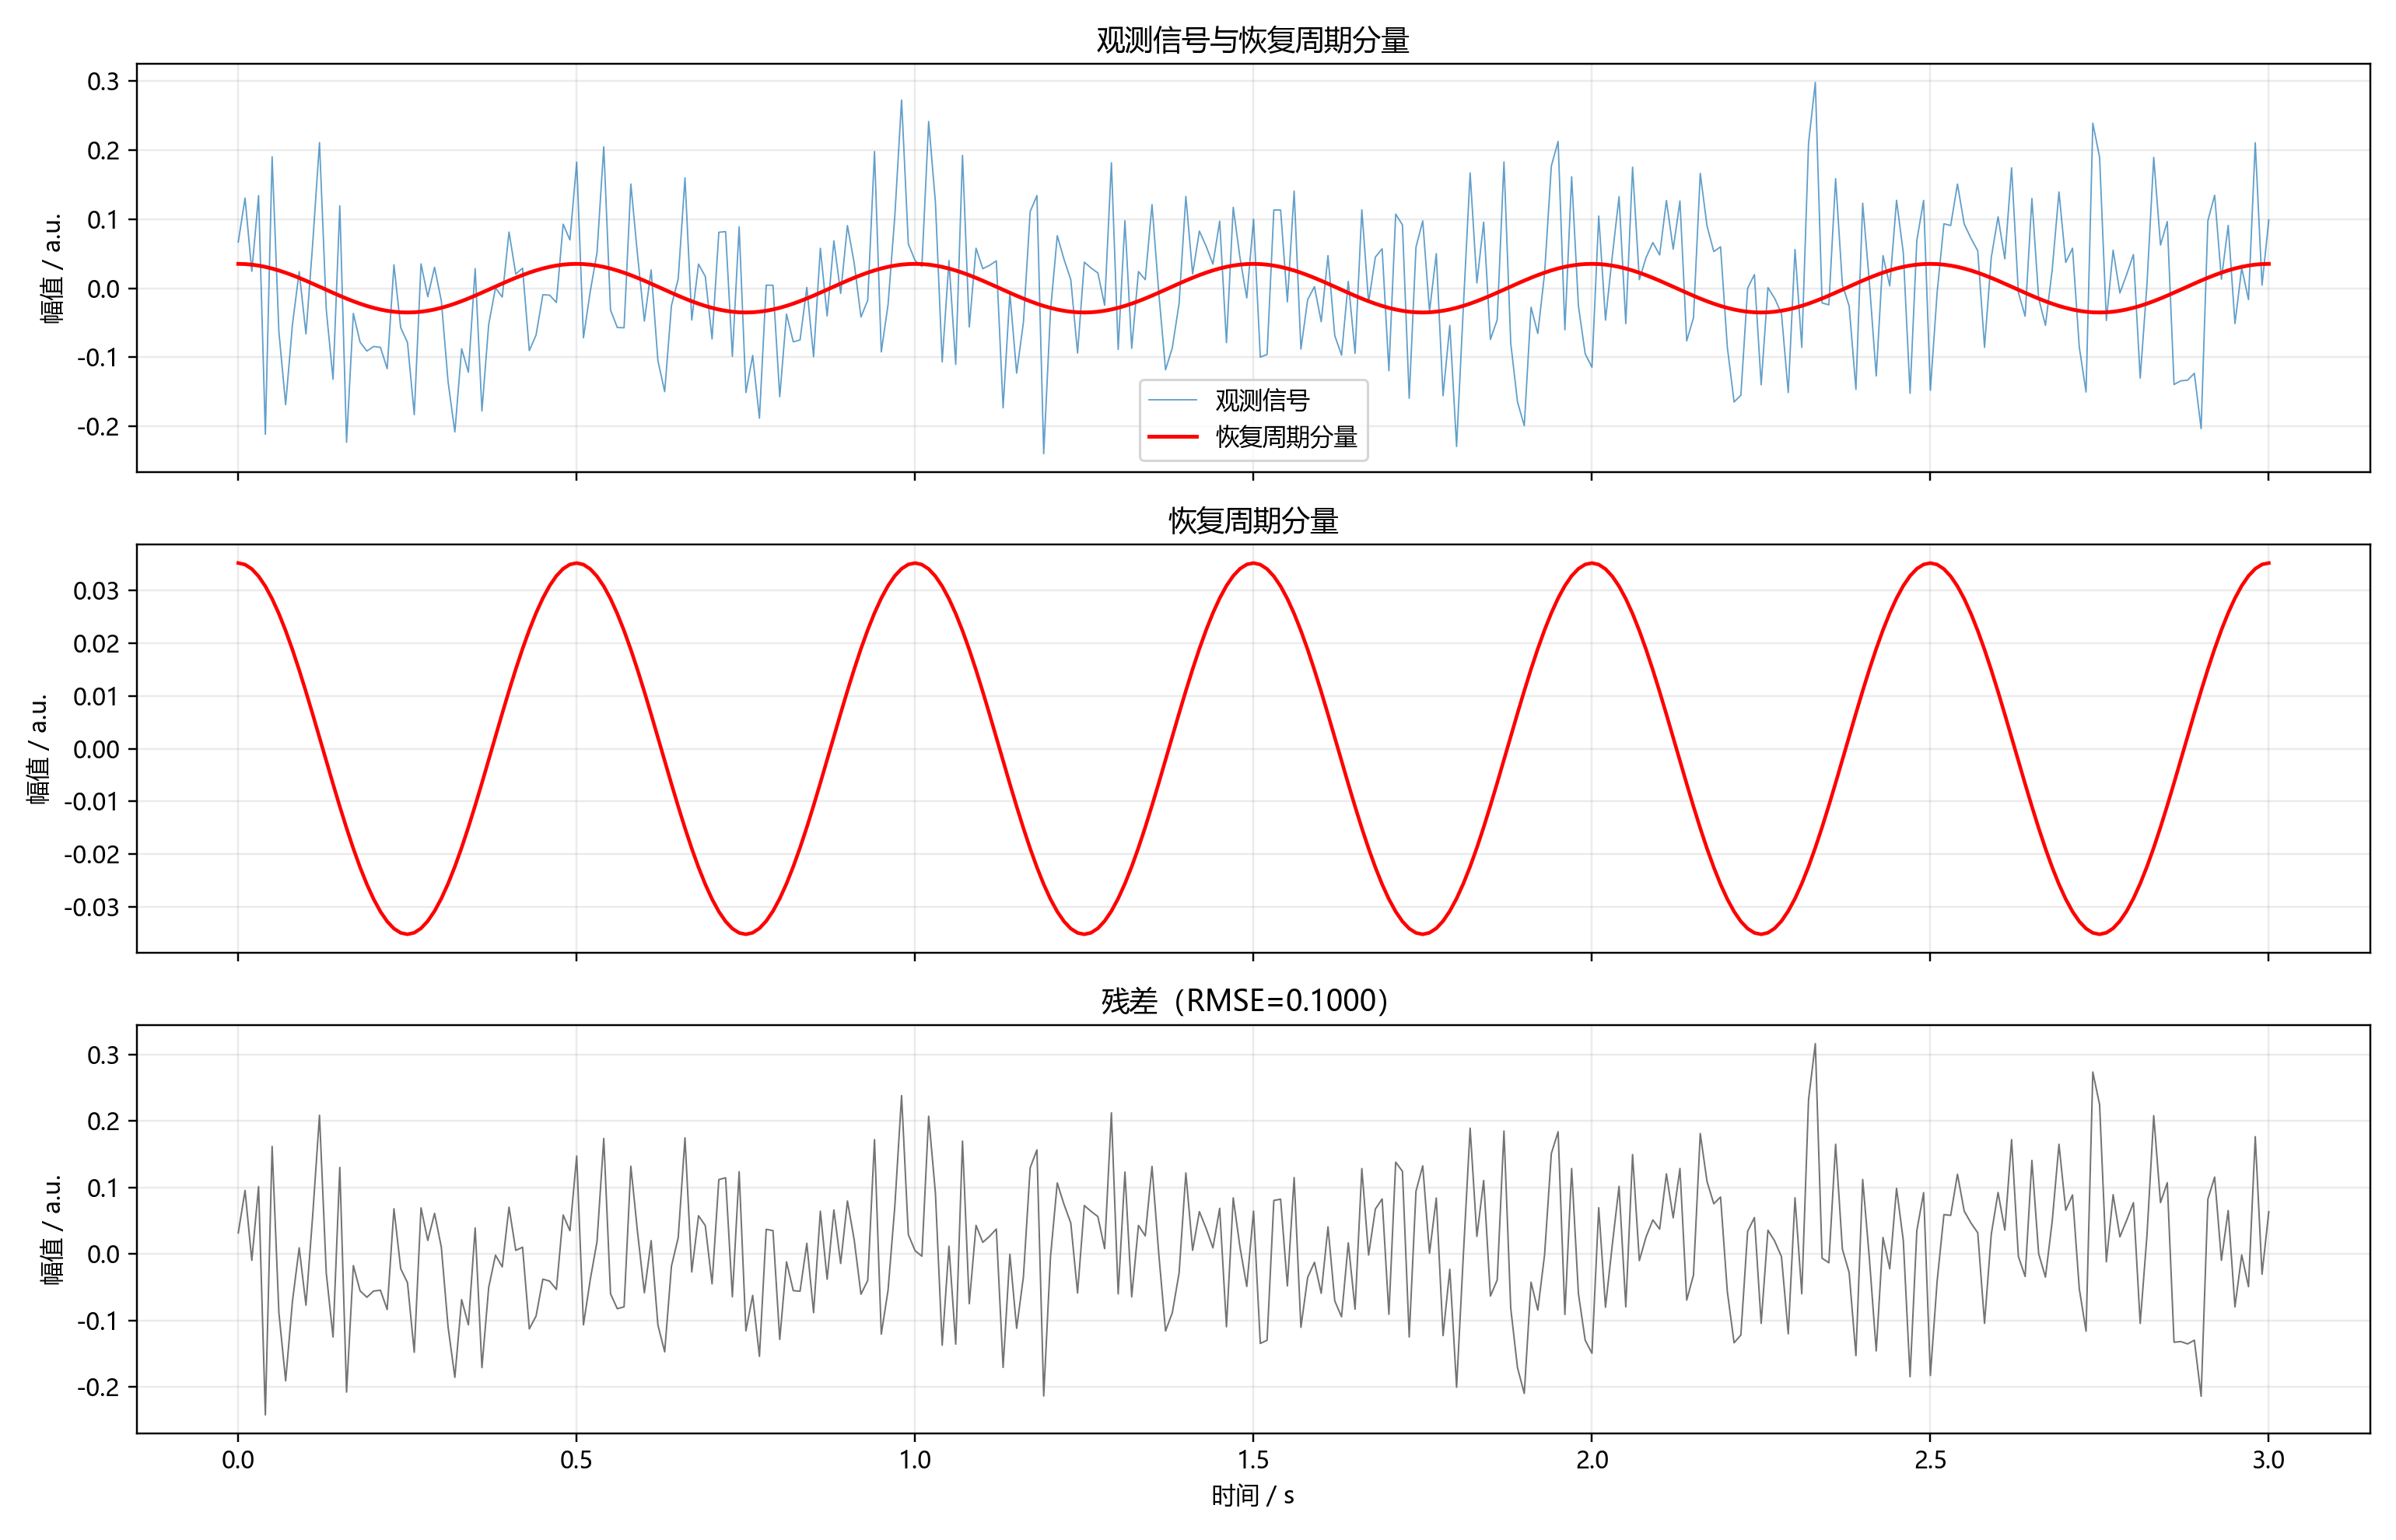
\includegraphics[width=0.90\textwidth,height=0.60\textheight,keepaspectratio]{figures/图3.png}
    \caption{单源故障信号恢复与残差}
    \label{fig:q2recovery}
\end{figure}

\begin{table}[H]
\centering
\normalsize
\setlength{\tabcolsep}{4pt}
\renewcommand{\arraystretch}{1.2}
\caption{单源故障波形恢复结果}
\label{tab:q2result}
\begin{tabular}{>{\centering\arraybackslash}m{3.2cm} >{\centering\arraybackslash}m{3.5cm} m{7cm}}
\toprule
指标 & 估计值 & 解释 \\
\midrule
故障频率 \(f_0\) & \(2.0000\,\mathrm{Hz}\) & 由 FFT 精细定位并经 Welch 验证 \\
振幅 \(A\) & \(0.0352\,\mathrm{a.u.}\) & 约为残差标准差的 \(35\%\) \\
初相 \(\varphi_0\) & \(1.574\,\mathrm{rad}\) & 约为 \(90.2^\circ\)，接近余弦形态 \\
残差 \(\mathrm{RMSE}\) & 0.1000 & 表征未解释部分，不是真实波形误差 \\
\(A\) 的条件 \(95\%\) CI & \([0.0338,0.0366]\,\mathrm{a.u.}\) & 条件于已估频率及白噪声近似 \\
\(\varphi_0\) 的条件 \(95\%\) CI & \([1.534,1.613]\,\mathrm{rad}\) & 不包含频率搜索的不确定性 \\
\bottomrule
\end{tabular}
\end{table}

表~\ref{tab:q2result} 中的区间是条件于已估频率和高斯白噪声近似的参数区间；其用途是量化回归系数不确定性，而不是覆盖频率搜索及模型失配的完整置信区间。

为补足附件缺少无噪声真值的限制，本文以式~\eqref{eq:recovery} 为已知真值，从附件残差中有放回抽样构造同尺度噪声，重复500次“FFT连续峰值精化--最小二乘恢复”。表~\ref{tab:q2simulation} 给出各次误差的中位数及经验95\%区间；该实验验证算法在已知真值条件下的恢复能力，而不把合成真值冒充附件真实故障波形。

\begin{table}[H]
\centering
\small
\setlength{\tabcolsep}{4pt}
\renewcommand{\arraystretch}{1.15}
\caption{单源波形有真值仿真误差（500次）}
\label{tab:q2simulation}
\begin{tabular}{>{\centering\arraybackslash}m{4.5cm} >{\centering\arraybackslash}m{3.2cm} >{\centering\arraybackslash}m{4.2cm}}
\toprule
指标 & 中位数 & 经验95\%区间 \\
\midrule
频率绝对误差 / Hz & \(5.17\times10^{-5}\) & \([4.97,5.38]\times10^{-5}\) \\
振幅相对误差 & 1.38\% & 0.051\%--4.41\% \\
相位绝对误差 / rad & 0.0653 & 0.0257--0.1041 \\
波形NRMSE & 4.47\% & 3.76\%--6.44\% \\
\bottomrule
\end{tabular}
\end{table}

\begin{figure}[H]
    \centering
    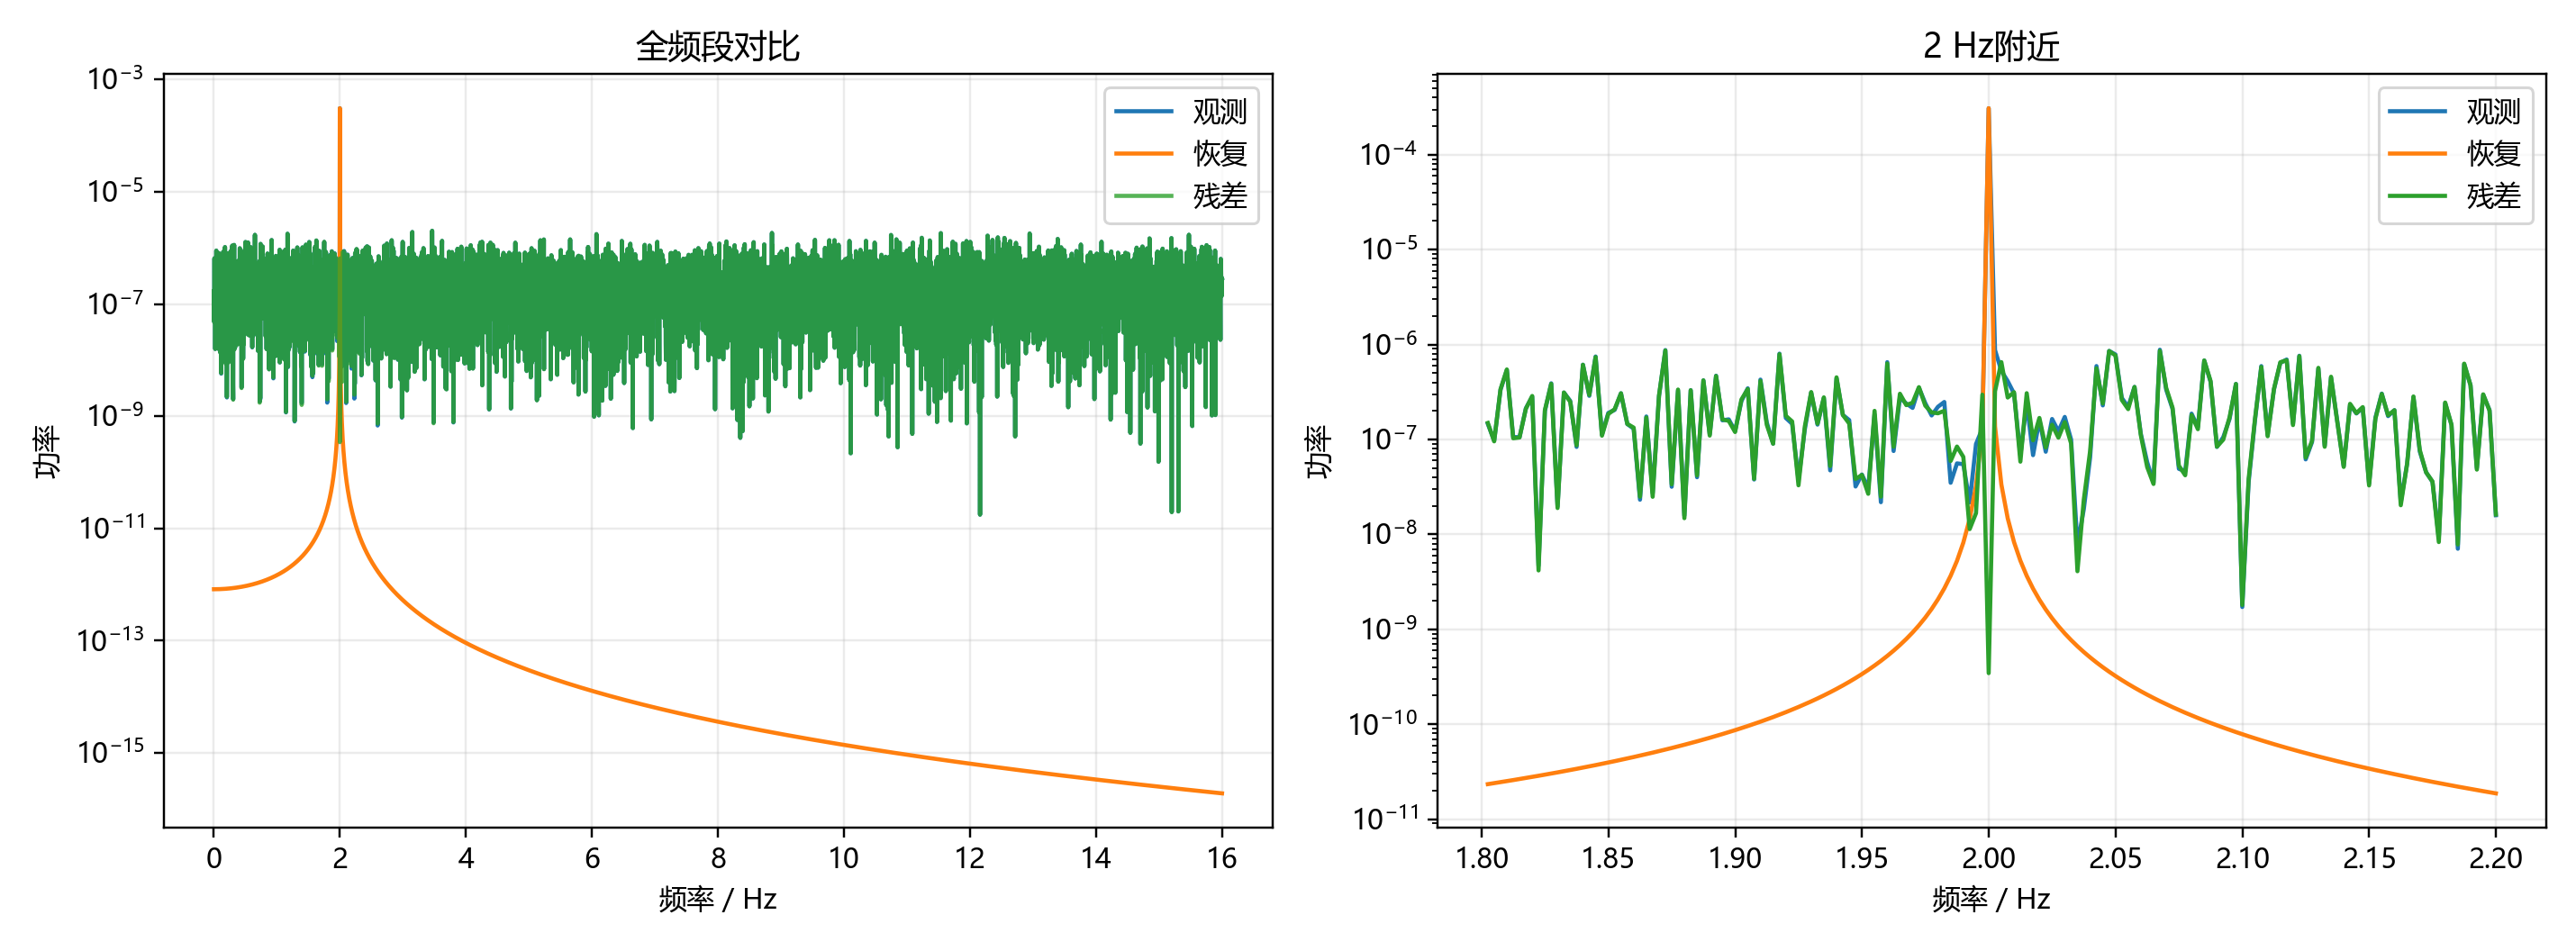
\includegraphics[width=0.90\textwidth,height=0.58\textheight,keepaspectratio]{figures/图4.png}
    \caption{信号恢复结果的频域对比}
    \label{fig:q2freq}
\end{figure}
图~\ref{fig:q2freq} 进一步表明，恢复分量的能量集中于2 Hz，残差在该频率附近未出现同量级窄带峰。

\subsection{问题三结果：多故障源分离}

对多源信号应用宽松寻峰与 \(\mathrm{BIC}\) 自动选阶，\(\mathrm{BIC}\) 在 \(M=4\) 处取得最小值；\(\mathrm{BIC}(5)-\mathrm{BIC}(4)=13.36\)，表明增加第五个分量所得残差改善不足以抵消复杂度惩罚。在固定候选峰集合下进行500次条件残差Bootstrap，四阶模型被选择500次，选阶比例为100\%；该结果证明选阶对残差扰动稳定，但不覆盖候选峰提取规则改变带来的不确定性。

\begin{table}[H]
\centering
\normalsize
\setlength{\tabcolsep}{4pt}
\renewcommand{\arraystretch}{1.25}
\caption{多故障源联合最小二乘估计结果}
\label{tab:q3result}
\begin{tabular}{>{\centering\arraybackslash}m{2.4cm} >{\centering\arraybackslash}m{2cm} >{\centering\arraybackslash}m{2.4cm} >{\centering\arraybackslash}m{2cm} m{4.2cm}}
\toprule
\shortstack{故障频率\\\(f_i/\mathrm{Hz}\)} & \shortstack{振幅\\\(A_i\)} & \shortstack{初相\\\(\varphi_i/\mathrm{rad}\)} & \shortstack{初相\\\(/\,{}^\circ\)} & 工程解释 \\
\midrule
4.0000 & 0.0191 & 1.372 & 78.6 & 低频分量 \\
7.9999 & 0.0249 & -2.989 & -171.3 & 第二分量 \\
13.0001 & 0.0105 & -2.157 & -123.6 & 最弱分量 \\
14.0000 & 0.0401 & 0.112 & 6.4 & 最强分量 \\
\bottomrule
\end{tabular}
\end{table}

从表~\ref{tab:q3result} 可见，数据支持四阶周期模型，但这并不等同于已知真实物理源数。图~\ref{fig:q3bic} 给出了 FFT 候选峰及 \(\mathrm{BIC}\) 选阶曲线。

\begin{figure}[H]
    \centering
    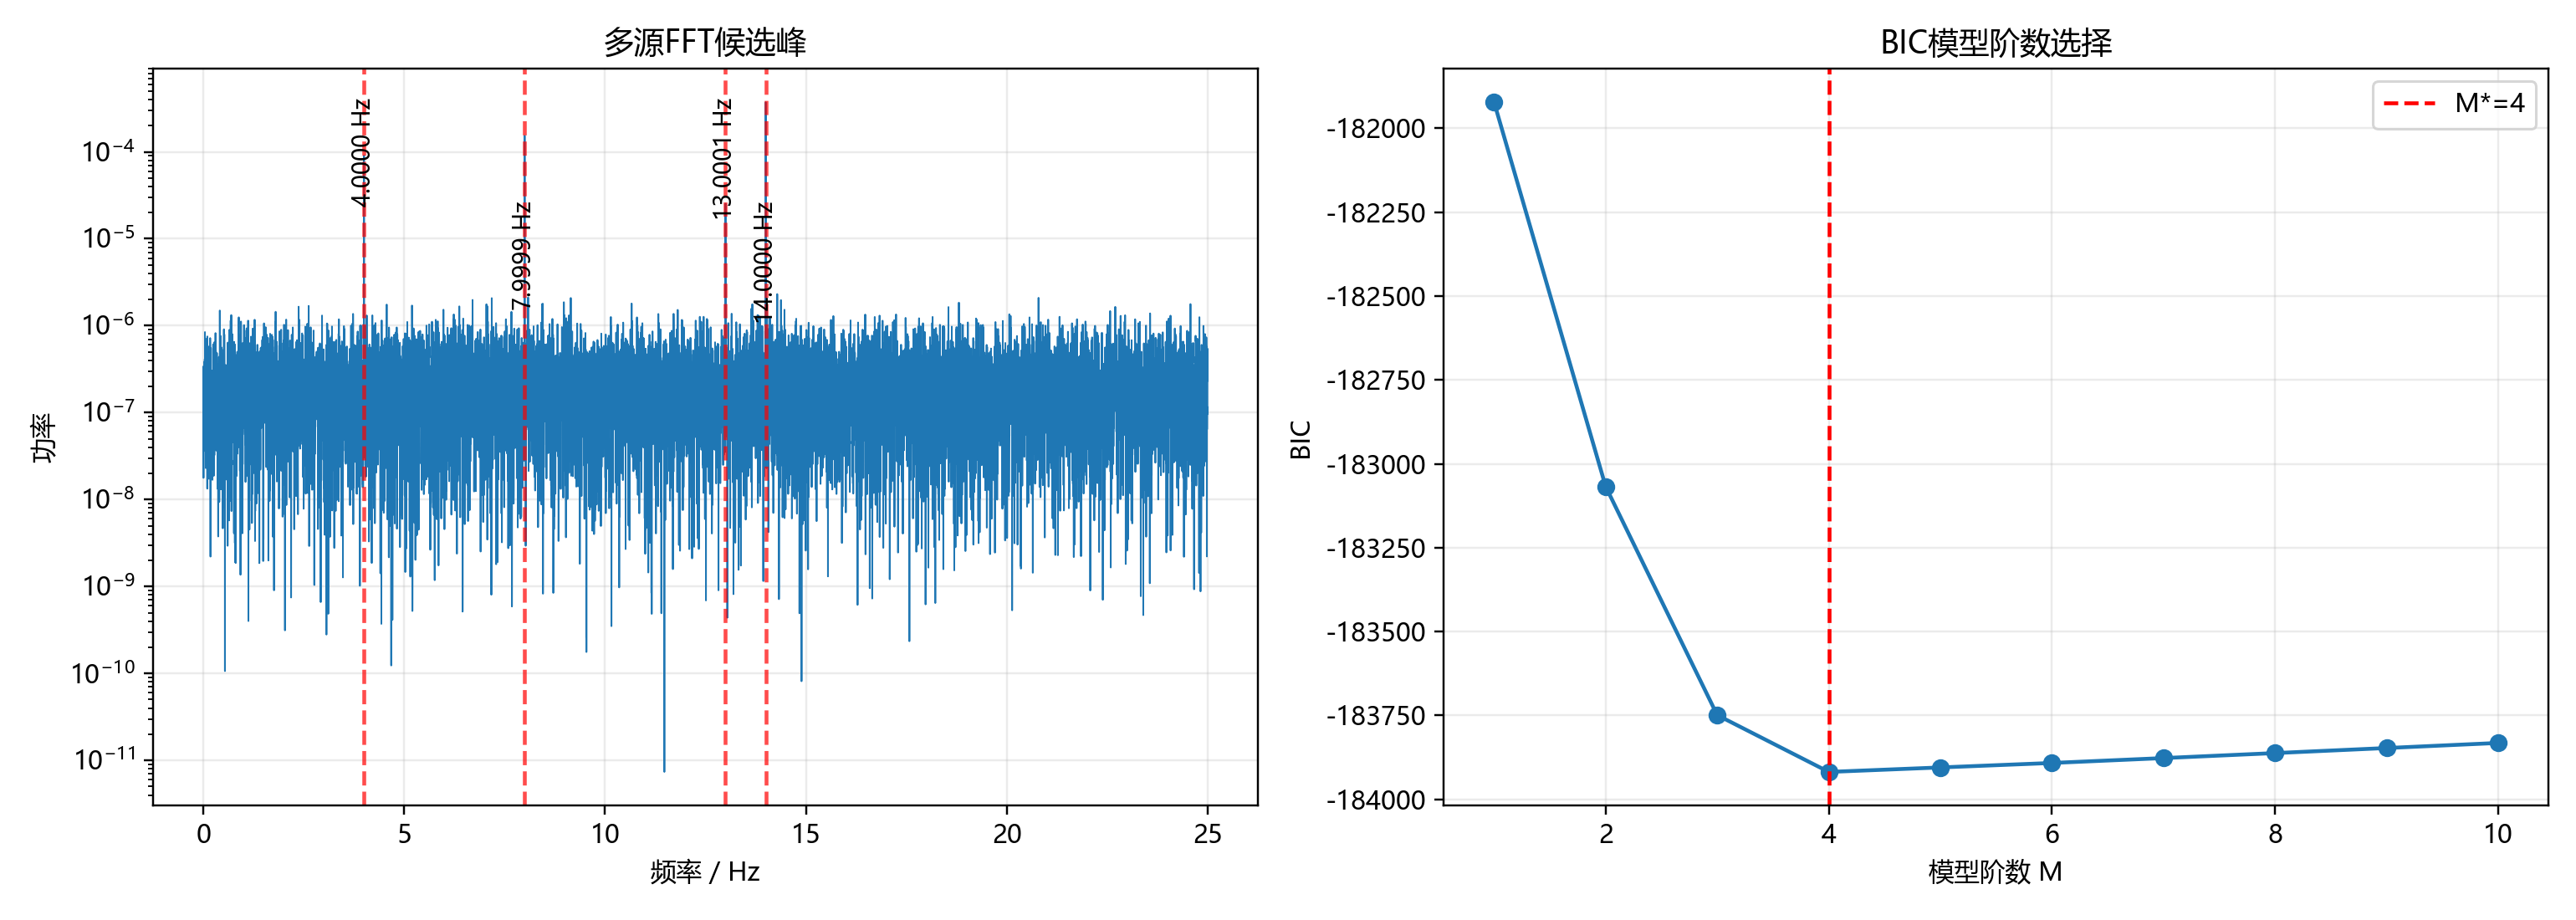
\includegraphics[width=0.90\textwidth,height=0.58\textheight,keepaspectratio]{figures/图5.png}
    \caption{多源频谱寻峰与 \(\mathrm{BIC}\) 选阶}
    \label{fig:q3bic}
\end{figure}

在多源时域分离中，采用连续频率联合最小二乘重建四个周期分量。如图~\ref{fig:q3sep} 所示，本文分离的是可辨识的周期分量，不把它们过度解释为已完成物理源定位。

\begin{figure}[H]
    \centering
    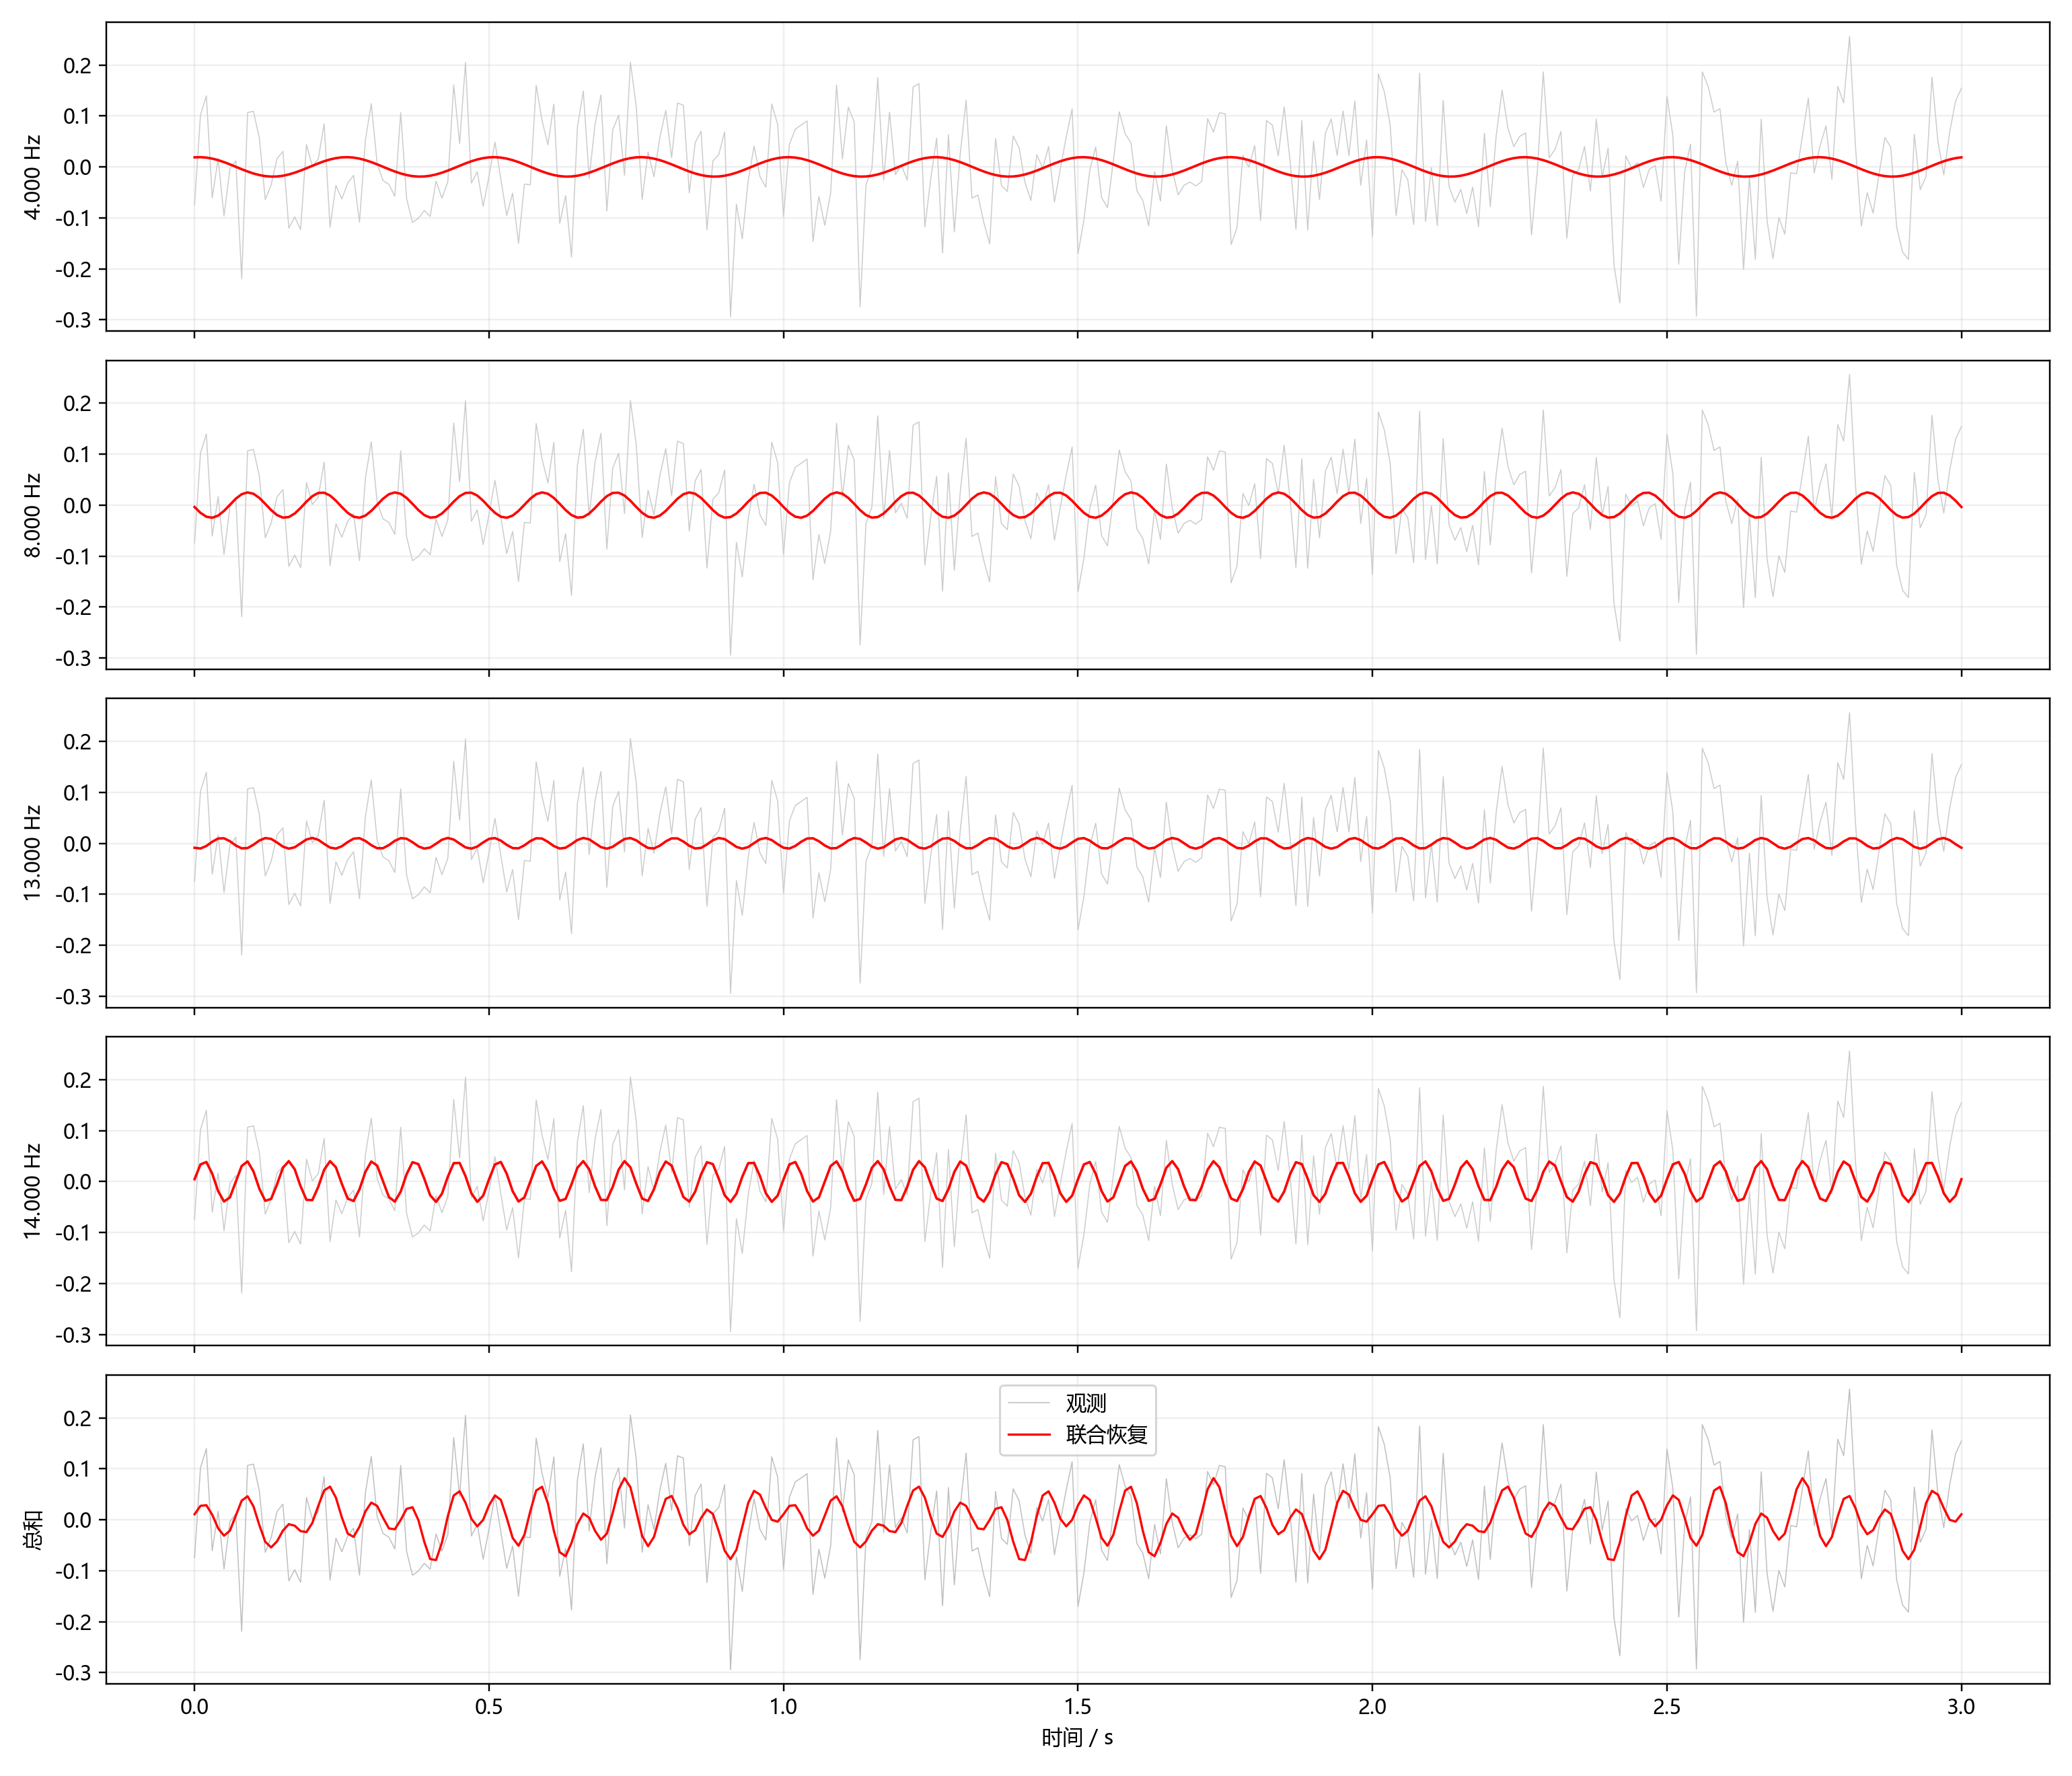
\includegraphics[width=0.86\textwidth,height=0.62\textheight,keepaspectratio]{figures/图6.png}
    \caption{多故障源时域波形分离}
    \label{fig:q3sep}
\end{figure}

多频率联合恢复后的残差 \(\mathrm{RMSE}\) 为 \(0.0999\)。图~\ref{fig:q3limit} 所示的500次蒙特卡洛实验表明：间隔 \(0.0025\,\mathrm{Hz}\) 时成功率为6.6\%，Wilson 95\%区间为4.74\%--9.12\%；间隔达到 \(0.005\,\mathrm{Hz}\) 后500次均成功，对应成功概率的Wilson 95\%区间为99.24\%--100\%，故本文数据条件下的经验分辨界约为 \(0.005\,\mathrm{Hz}\)，而实际最小间距为1 Hz。该结论是给定振幅、相位分布和噪声条件下的经验界，不宣称为普适理论极限。

\begin{figure}[H]
    \centering
    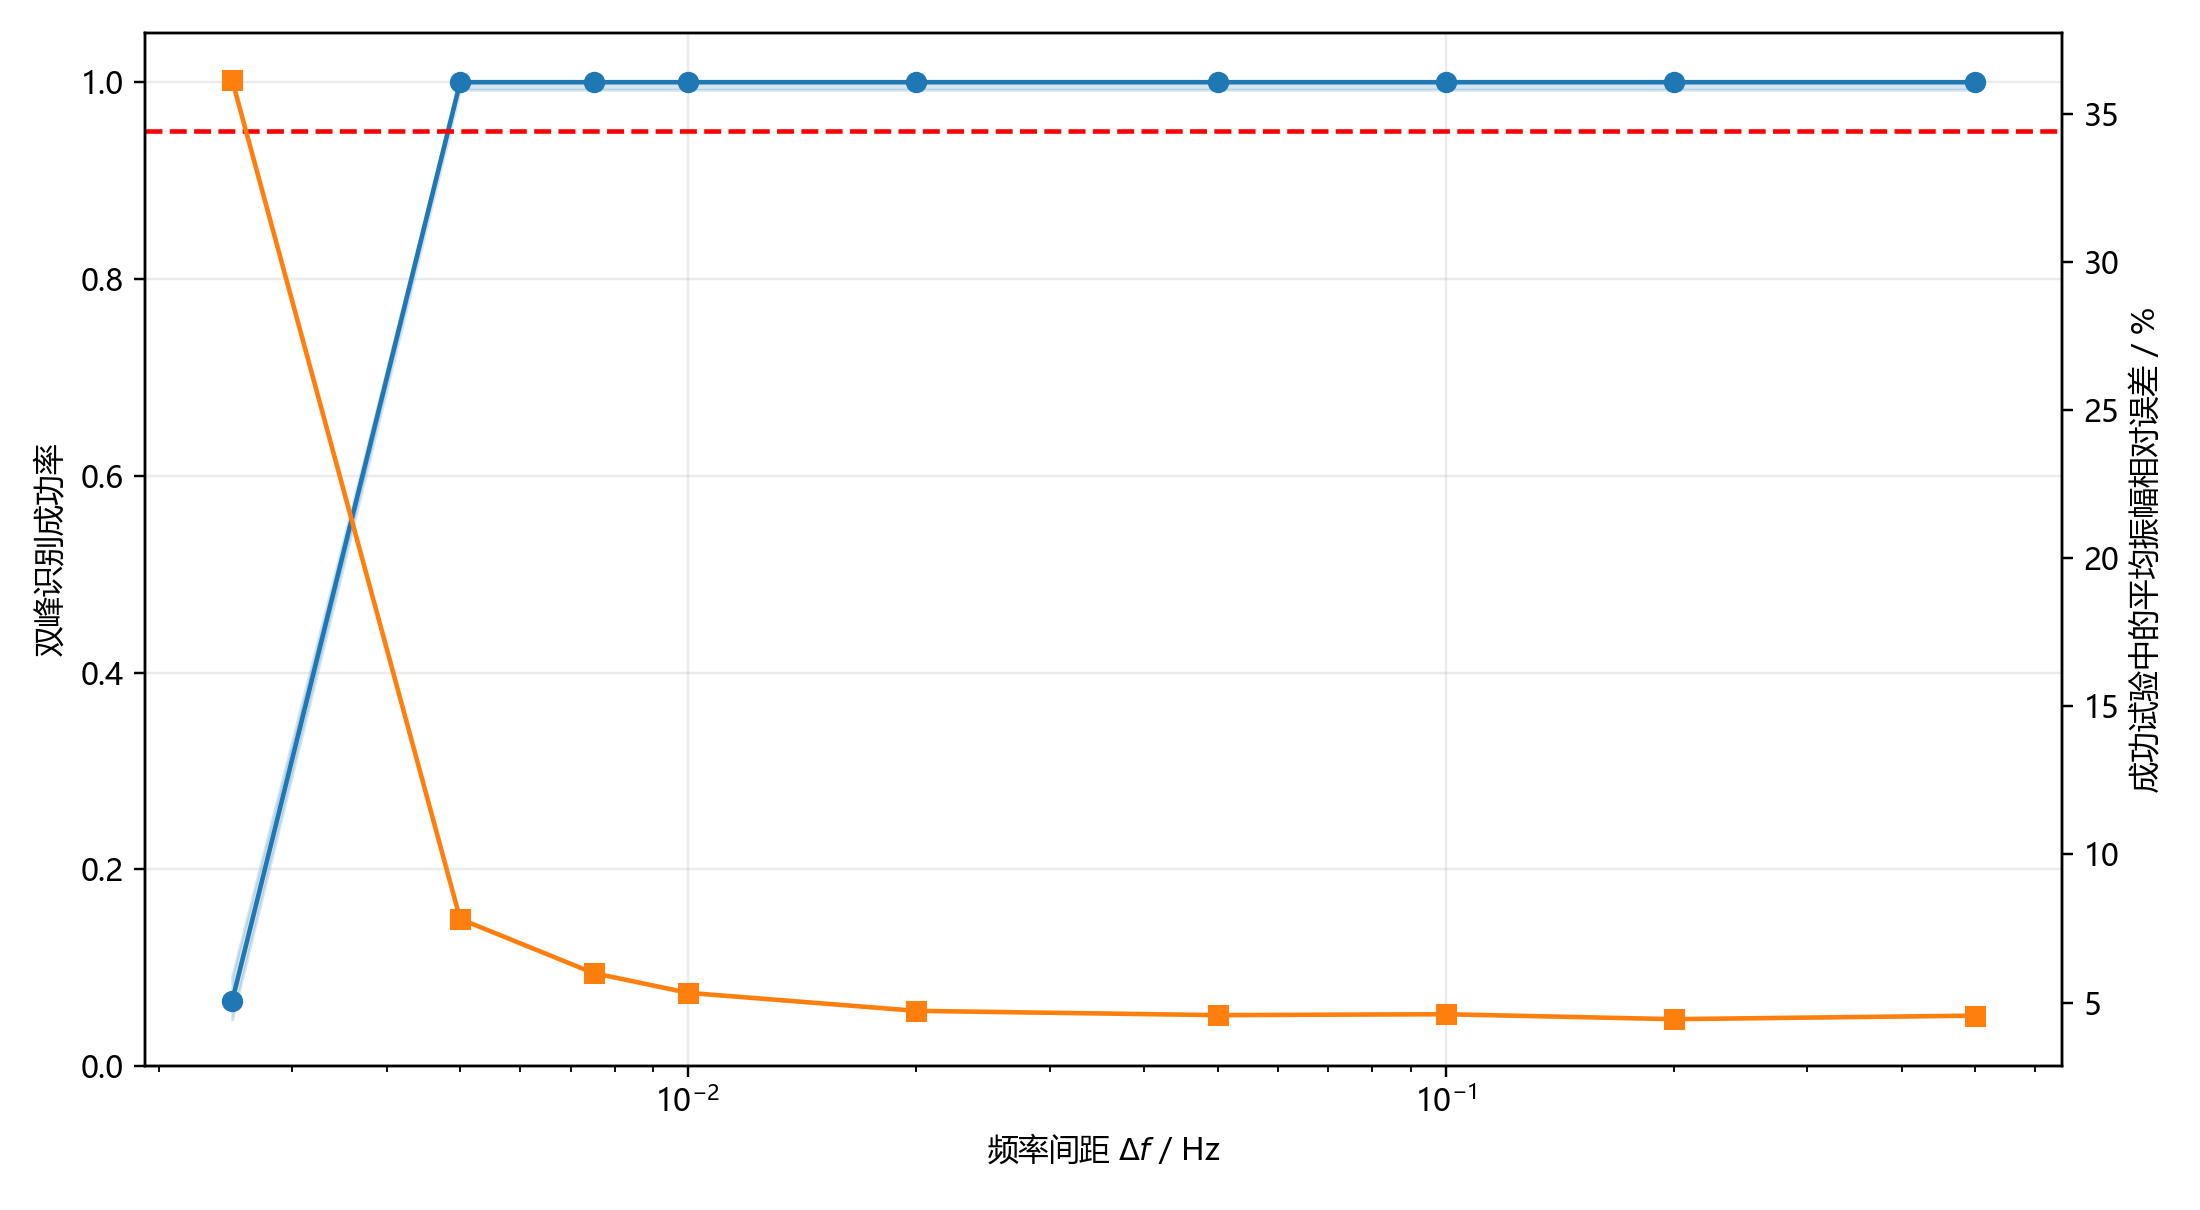
\includegraphics[width=0.84\textwidth,height=0.55\textheight,keepaspectratio]{figures/图7.png}
    \caption{相邻双频分辨实验}
    \label{fig:q3limit}
\end{figure}

\subsection{问题四结果：传感器布局优化}

在代表性算例的 \(0.25\,\mathrm{m}\) 网格上穷举 \(187460\) 种三传感器组合。名义评估取 \(\alpha=0.5\)、基准噪声0.1000并设中心附近噪声升高35\%、\(g_{ij}=1\)；布局设计则采用最弱振幅0.0105、\(\alpha=0.8\)、噪声尺度1.2和 \(g_{ij}=0.85\) 的不利组合。图~\ref{fig:q4layout} 和表~\ref{tab:q4layout} 给出该代表性场景的鲁棒布点。真实设备应用时须将算例几何和参数替换为图纸及标定数据后重新运行算法。

\begin{figure}[H]
    \centering
    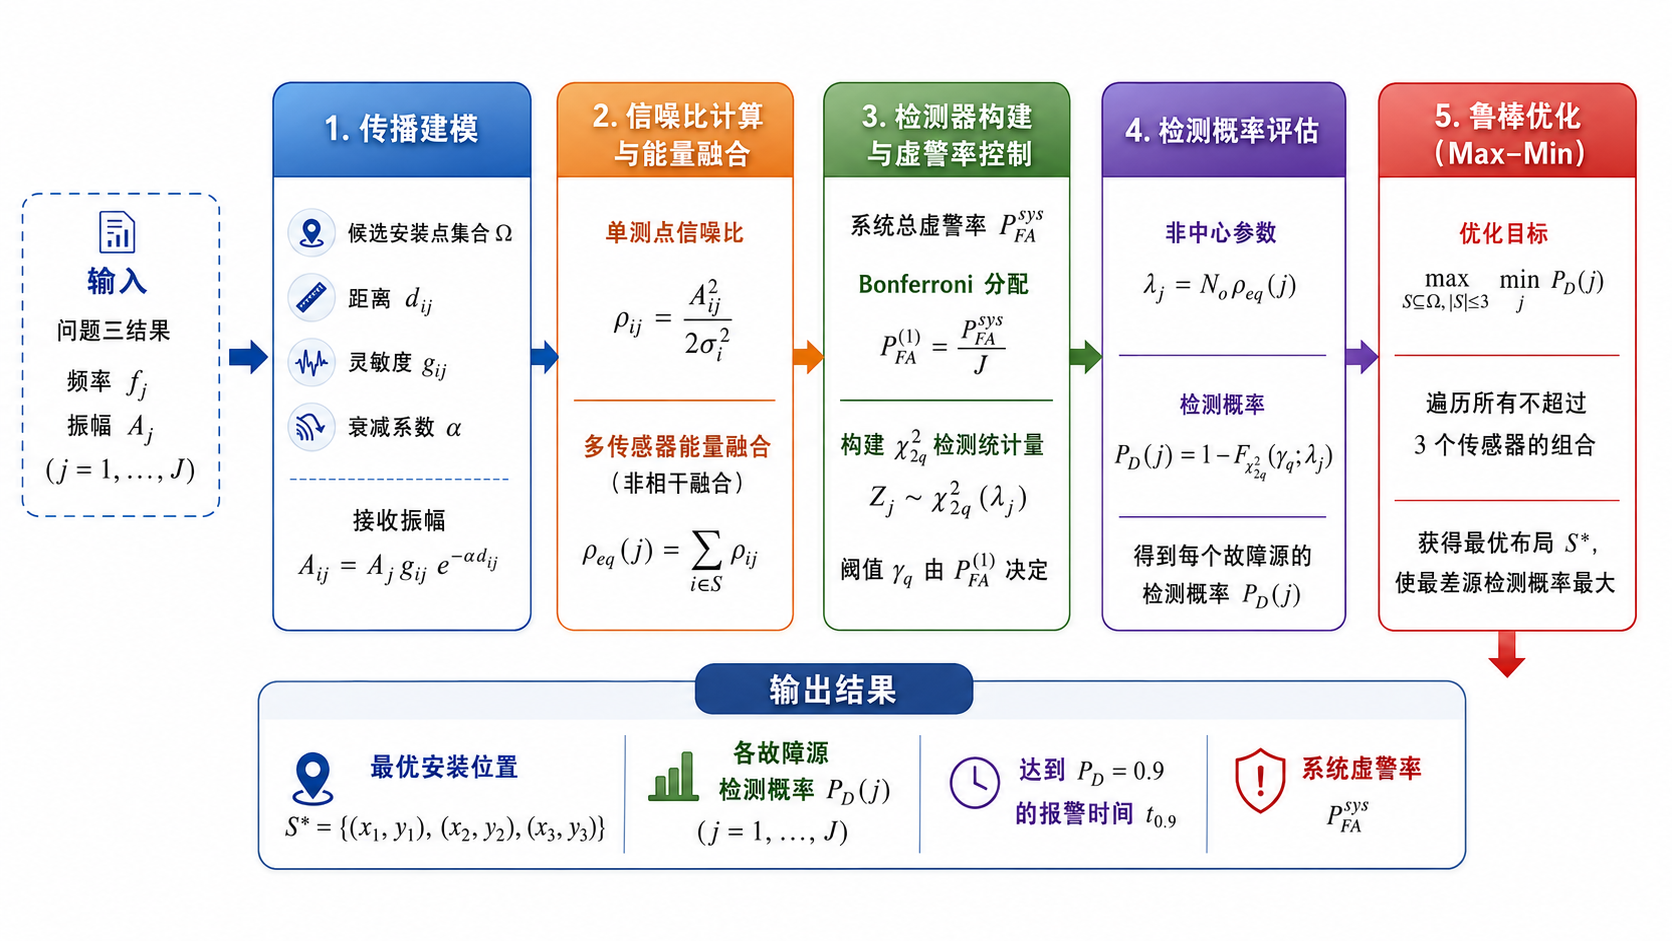
\includegraphics[width=0.98\textwidth]{figures/图9 .png}
    \caption{问题四传感器布局优化流程图}
    \label{fig:q4flow}
\end{figure}

\begin{figure}[H]
    \centering
    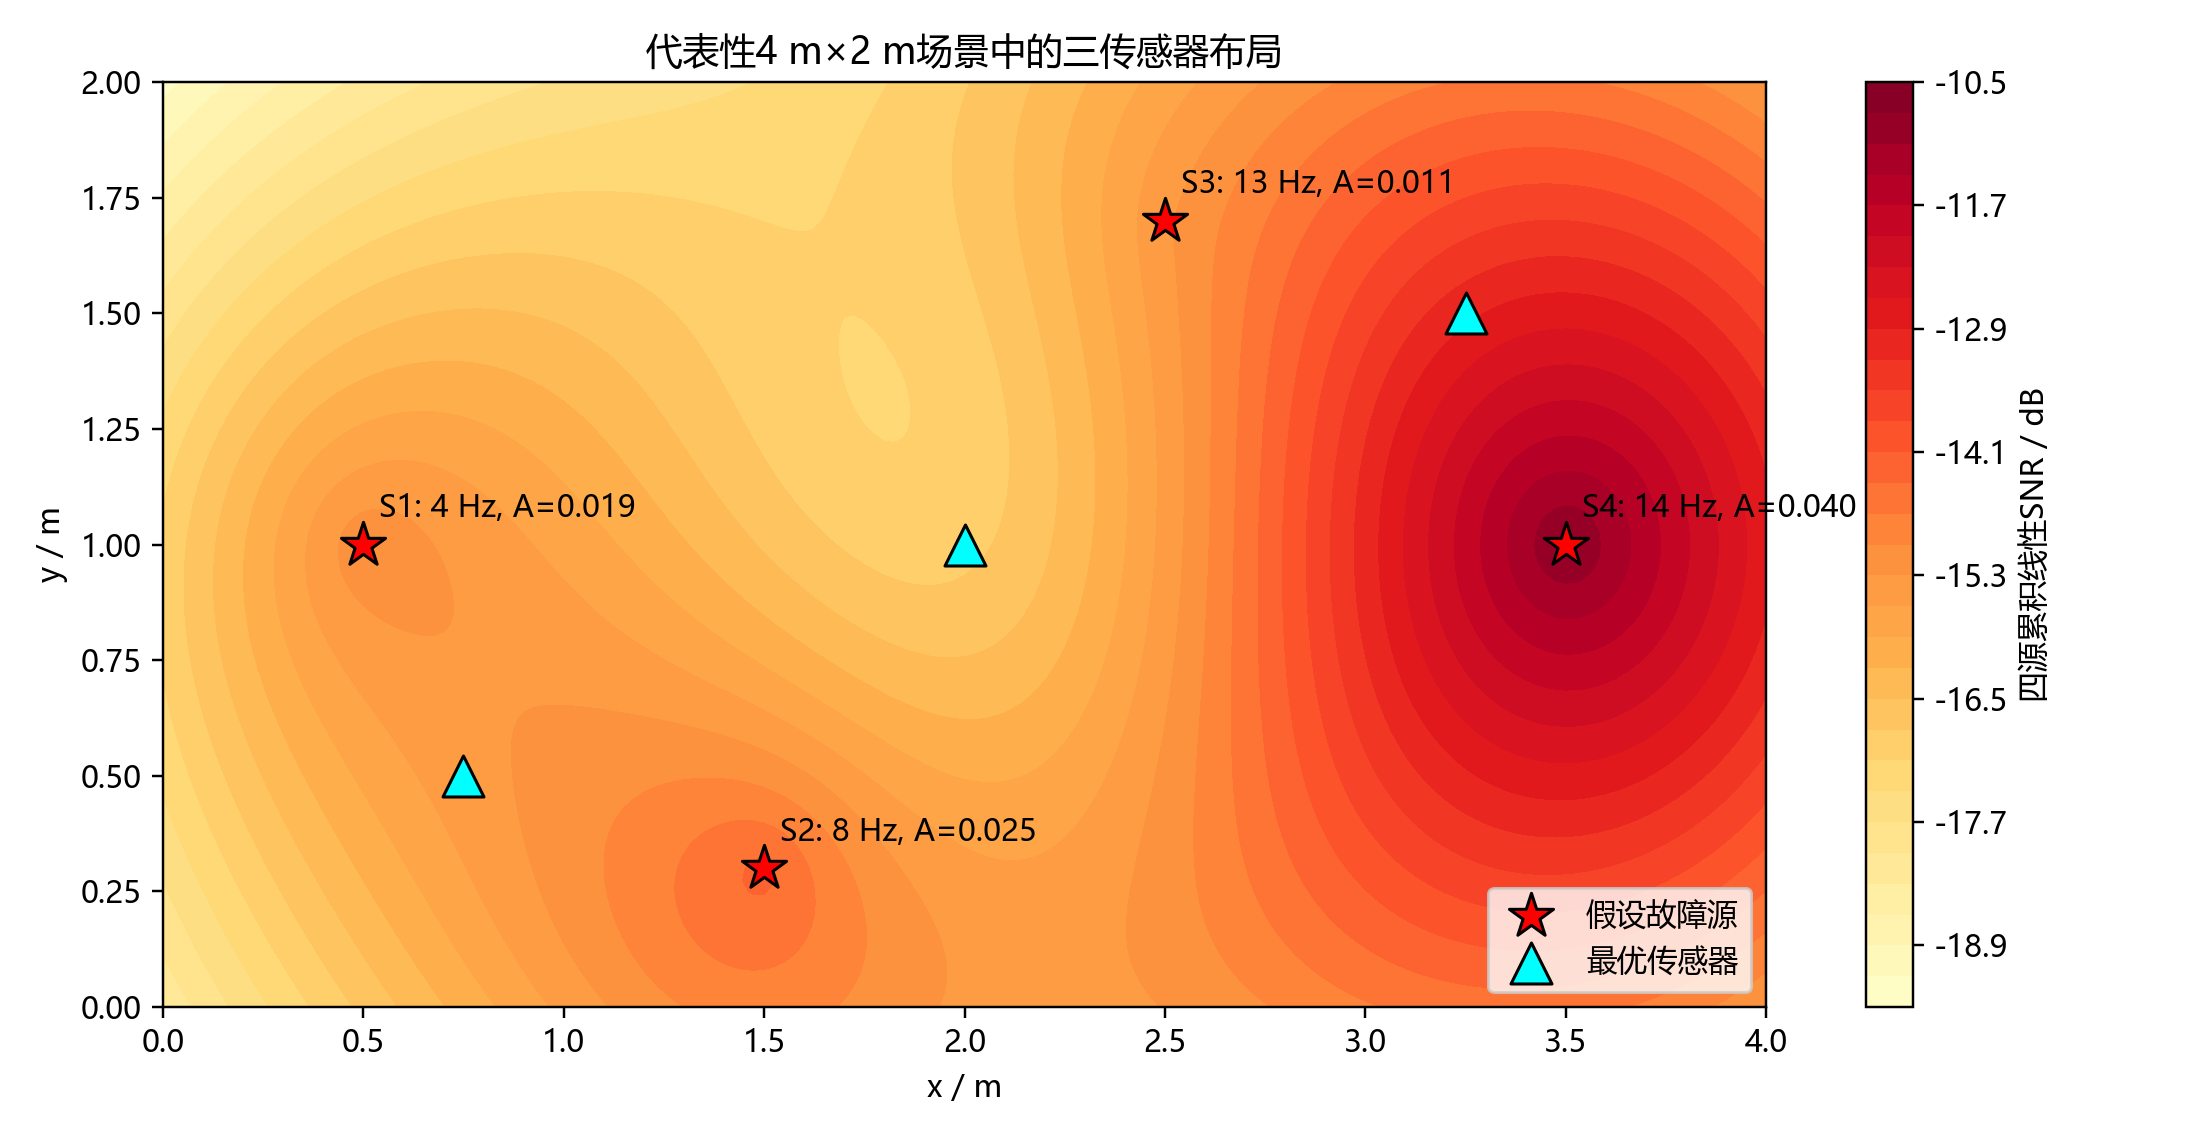
\includegraphics[width=0.84\textwidth,height=0.58\textheight,keepaspectratio]{figures/图8.png}
    \caption{代表性算例的鲁棒布局}
    \label{fig:q4layout}
\end{figure}

\begin{table}[H]
\centering
\normalsize
\setlength{\tabcolsep}{4pt}
\renewcommand{\arraystretch}{1.25}
\caption{代表性算例的鲁棒三传感器布局}
\label{tab:q4layout}
\begin{tabular}{>{\centering\arraybackslash}m{1.5cm} >{\centering\arraybackslash}m{3.2cm} m{5cm} >{\centering\arraybackslash}m{2.8cm}}
\toprule
编号 & 安装坐标 / m & 设计作用 & 备注 \\
\midrule
T1 & \((0.75,0.50)\) & 覆盖左侧潜在源 & 代表性算例坐标 \\
T2 & \((2.00,1.00)\) & 覆盖中部潜在源 & 代表性算例坐标 \\
T3 & \((3.25,1.50)\) & 覆盖右侧潜在源 & 代表性算例坐标 \\
\bottomrule
\end{tabular}
\end{table}

\begin{table}[H]
\centering
\normalsize
\setlength{\tabcolsep}{4pt}
\renewcommand{\arraystretch}{1.25}
\caption{传感器数量对检测性能的影响}
\label{tab:q4compare}
\begin{tabular}{>{\centering\arraybackslash}m{3.5cm} >{\centering\arraybackslash}m{3cm} >{\centering\arraybackslash}m{3cm} >{\centering\arraybackslash}m{2.5cm}}
\toprule
方案 & 最差源 \(\mathrm{SNR}\) & 最差 \(P_D\)（4 s） & 达到 \(P_D=0.9\) 的时间 \\
\midrule
鲁棒最优 1 传感器 & \(-30.151\,\mathrm{dB}\) & 0.0060 & 220.7 s \\
鲁棒最优 2 传感器 & \(-24.930\,\mathrm{dB}\) & 0.0121 & 77.8 s \\
鲁棒最优 3 传感器 & \(-23.661\,\mathrm{dB}\) & \textbf{0.0132} & \textbf{64.4 s} \\
\bottomrule
\end{tabular}
\end{table}

表~\ref{tab:q4compare} 汇总不同传感器数量下的名义性能。图~\ref{fig:q4roc} 分别给出以系统总虚警率为横轴的 ROC 曲线，以及故障功率尺度变化下的最差检测概率。三传感器方案的排序保持领先，但短时弱源检测仍然困难，不能把“相对改善”夸写成“已高概率检出”。

\begin{figure}[H]
    \centering
    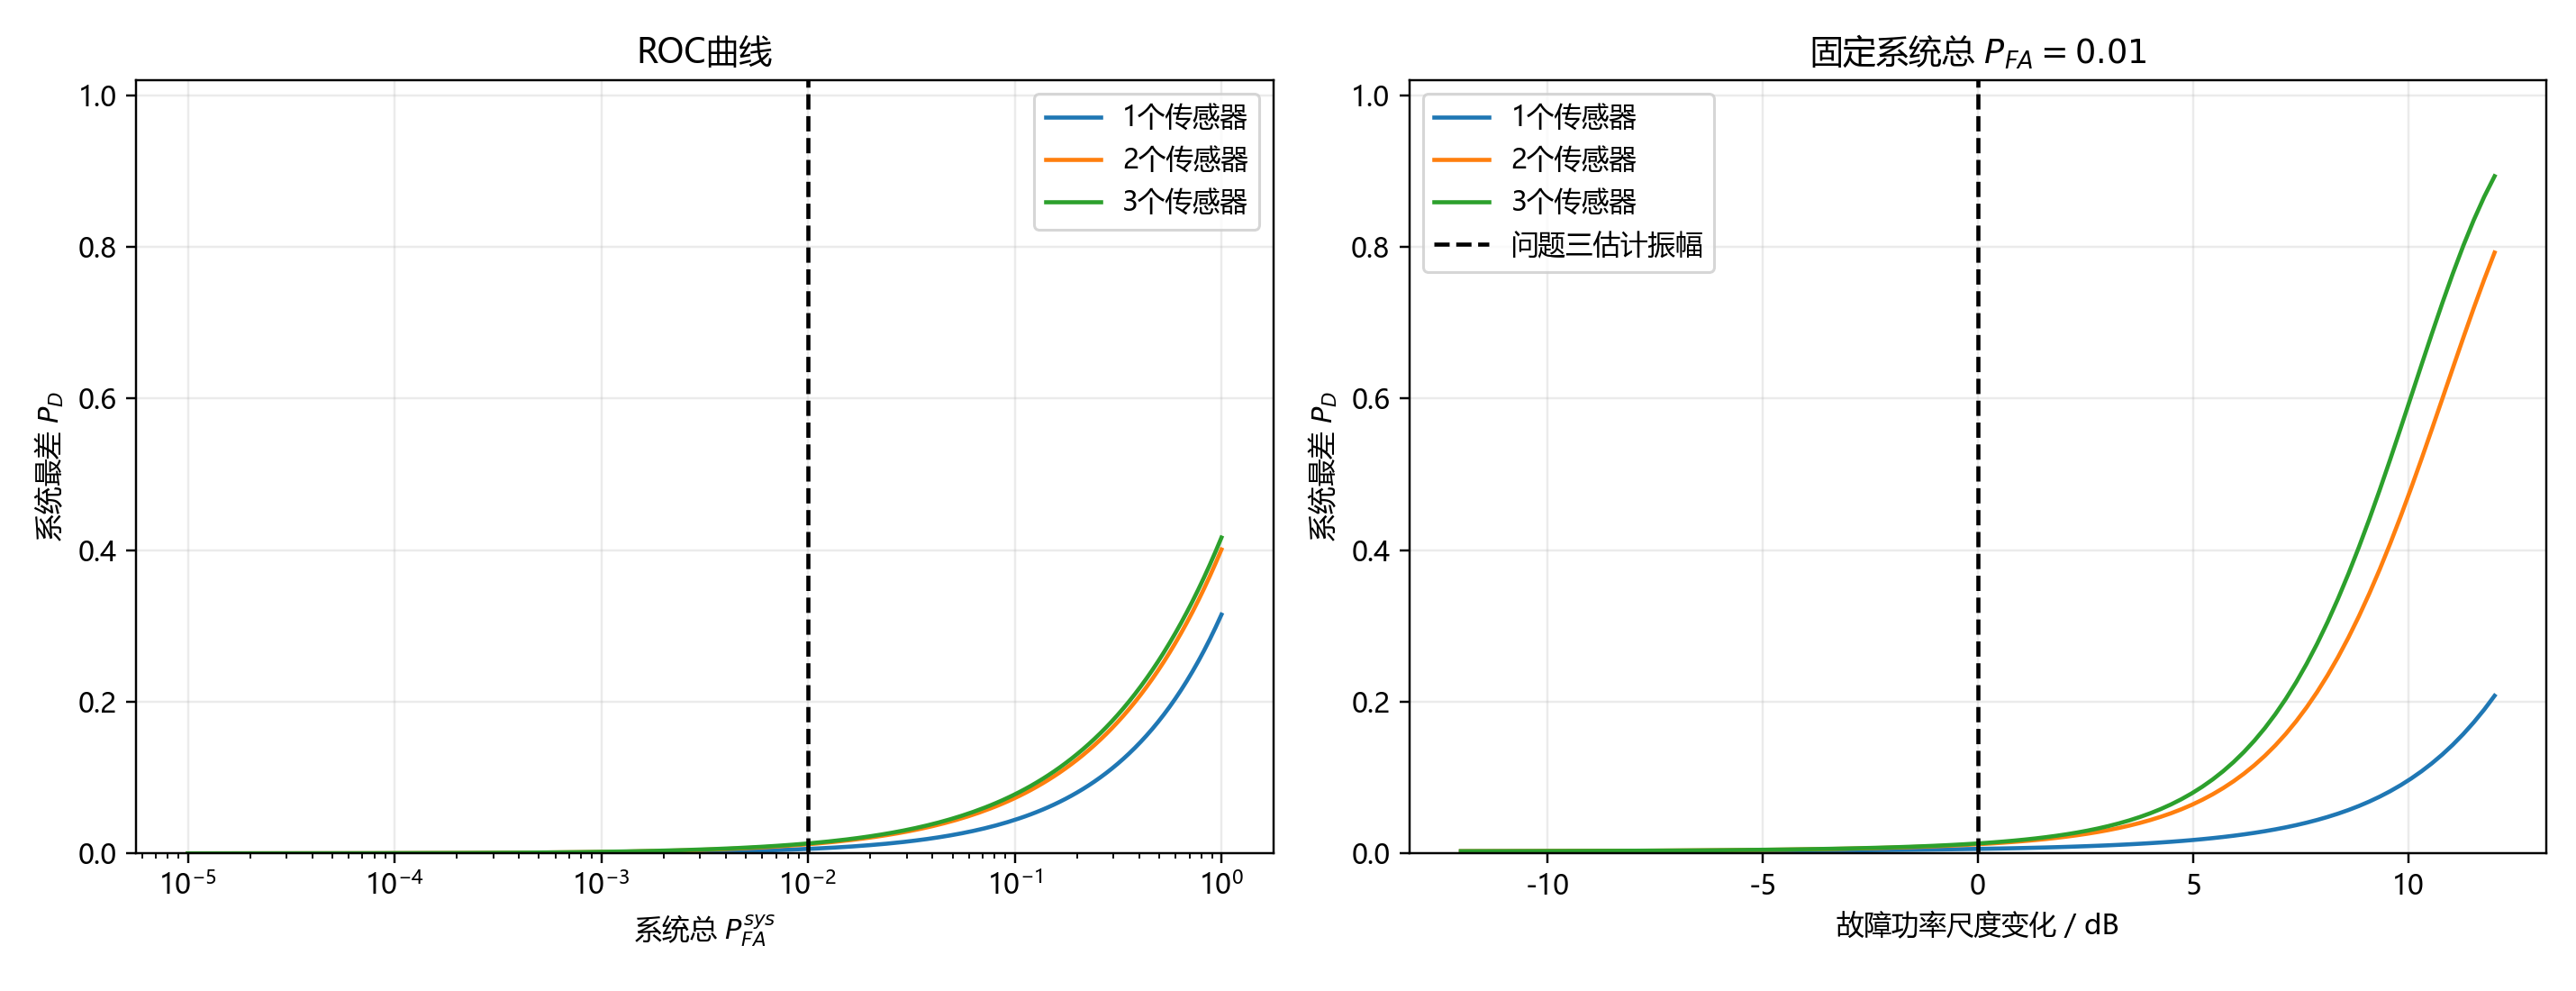
\includegraphics[width=0.90\textwidth,height=0.58\textheight,keepaspectratio]{figures/图10.png}
    \caption{系统ROC与故障功率敏感性}
    \label{fig:q4roc}
\end{figure}

结果表明，三传感器通过空间分集改善最弱覆盖：系统总 \(P_{FA}^{\mathrm{sys}}=0.01\)、4 s观测时，最差 \(P_D\) 由0.0060提高至0.0132；更有工程意义的是达到 \(P_D=0.9\) 的观测时间由220.7 s缩短至64.4 s。对四个振幅与四个位置的全部排列复核后，三点布局最差 \(P_D\) 位于0.0120--0.0132，说明保守布局对未知对应关系不敏感。

\subsubsection*{工程落地流程与有效性边界}

题目没有提供足以唯一确定物理坐标的设备图纸和多测点标定数据，因此本文不能把表~\ref{tab:q4layout} 的算例坐标解释为真实设备最终安装点。实际应用应按以下流程替换算例输入，而无须改变优化框架：
\begin{enumerate}[label=（\arabic*）,leftmargin=3em,itemsep=0pt,topsep=2pt,parsep=0pt]
    \item 根据设备图纸、安装可达性和安全距离建立真实候选点集合 \(\Omega_{\mathrm{real}}\)，并标注轴承座、齿轮箱壳体等关键区域；
    \item 在停机敲击或可控激励下测得各候选点到各潜在源的频率响应 \(H_{ij}(f_j)\)，以实测 \(|H_{ij}|\) 替代指数衰减中的 \(g_{ij}e^{-\alpha d_{ij}}\)；
    \item 在健康工况下同步采集多测点噪声，估计位置相关方差及跨测点协方差，并在相关噪声下采用协方差预白化；
    \item 将前三问得到的 \(A_j,f_j\)、系统总虚警率及上述标定量代入式~\eqref{eq:threshold}--\eqref{eq:maxmin}，重新搜索不超过三个安装点；
    \item 用未参与标定的多测点数据验证系统总虚警率和最差检测概率，若理论分布失配，则以健康残差 Bootstrap 标定联合阈值。
\end{enumerate}
\textbf{问题四最终布局方案：}对具有左右轴承支承和中部齿轮箱的典型旋转机械，三个传感器采用“左轴承座--齿轮箱壳体--右轴承座”的区域级分散布局；若设备结构不同，则将三者替换为沿主要传播路径分散的三个关键承载部位。每个区域优先选择背景噪声低、安装刚度高且对最弱故障频率响应最大的候选点。获得现场标定数据后，最终坐标唯一按
\[
 \mathcal S^*=\arg\max_{\mathcal S\subseteq\Omega_{\mathrm{real}},\,|\mathcal S|\le3}
 \min_j P_D^{(j)}(\mathcal S)
\]
确定。若某区域候选点的灵敏度或噪声不满足要求，算法允许将该点移至其他关键部位，故区域级建议不替代数据驱动的最终优化。

代表性算例验证的是布局优化与统计检测流程的可执行性，不构成对真实设备传播模型及最终安装坐标的验证。

\section{模型检验}

\subsection{衰减系数灵敏度}

由于衰减系数与噪声场均需实测标定，本文固定表~\ref{tab:q4layout} 的鲁棒布局，对 \(\alpha\) 和噪声尺度同时扰动，而不是在知道扰动结果后重新选点。表~\ref{tab:sensitivity} 给出噪声尺度为1时的结果。

\begin{table}[H]
\centering
\normalsize
\setlength{\tabcolsep}{4pt}
\renewcommand{\arraystretch}{1.25}
\caption{衰减系数灵敏度}
\label{tab:sensitivity}
\begin{tabular}{>{\centering\arraybackslash}m{3cm} >{\centering\arraybackslash}m{4cm} >{\centering\arraybackslash}m{4cm}}
\toprule
衰减系数 \(\alpha\) & 最差源 SNR/dB & 最差 \(P_D\) \\
\midrule
0.3 & -21.845 & 0.0232 \\
0.4 & -22.775 & 0.0171 \\
0.5 & -23.661 & 0.0132 \\
0.6 & -24.508 & 0.0105 \\
0.8 & -26.117 & 0.0073 \\
\bottomrule
\end{tabular}
\end{table}

衰减增强或噪声上升均会降低绝对检测概率，这说明布局效果依赖工程标定，不能脱离参数报告单一“最优坐标”。另令 \(g_{ij}\) 在 \([0.85,1.15]\) 独立扰动5000次，最差 \(P_D\) 的5\%、50\%、95\%分位数为0.0106、0.0132、0.0165。

\subsection{理论分布与蒙特卡洛核验}

系统总虚警率0.01经 Bonferroni 分配后，单频率虚警率为0.0025；若额外假设四个频率检验独立，Šidák值为0.002509。两种口径下三传感器4 s最差 \(P_D\) 分别为0.01315和0.01319，相差不足0.3\%，说明保守控制几乎不牺牲性能。在正交匹配滤波输出层进行 \(10^5\) 次蒙特卡洛校准，四频率同时监测的经验系统虚警率为0.00995，理论检测概率与模拟值一致。图~\ref{fig:q4mc} 验证的是阈值和检测器数值实现；由于缺少真实多测点数据，它不能验证指数传播模型本身。
\begin{figure}[H]
    \centering
    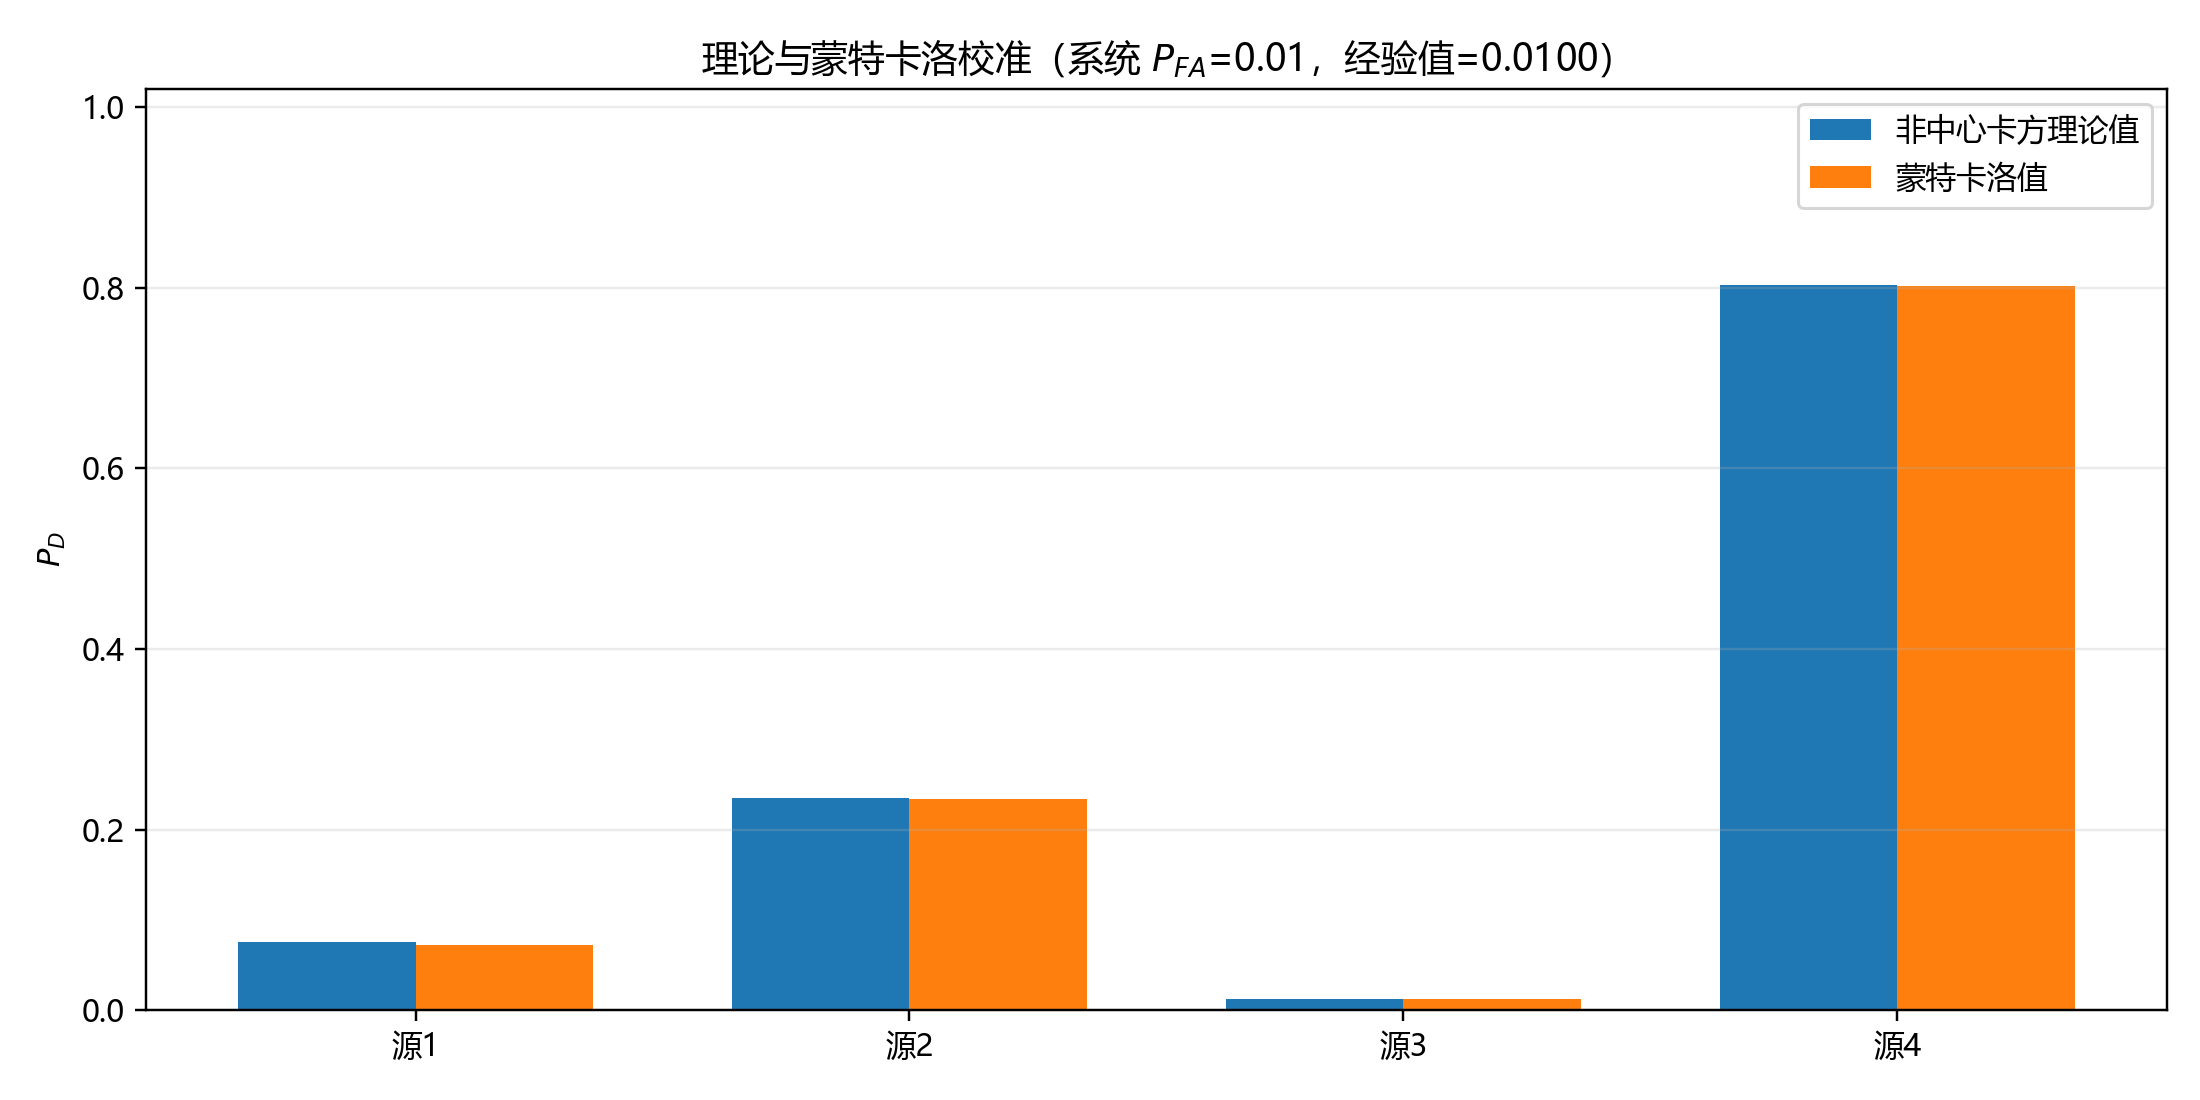
\includegraphics[width=0.84\textwidth]{figures/图11.png}
    \caption{理论值与蒙特卡洛核验}
    \label{fig:q4mc}
\end{figure}

\subsection{积累时长影响}

\begin{figure}[H]
    \centering
    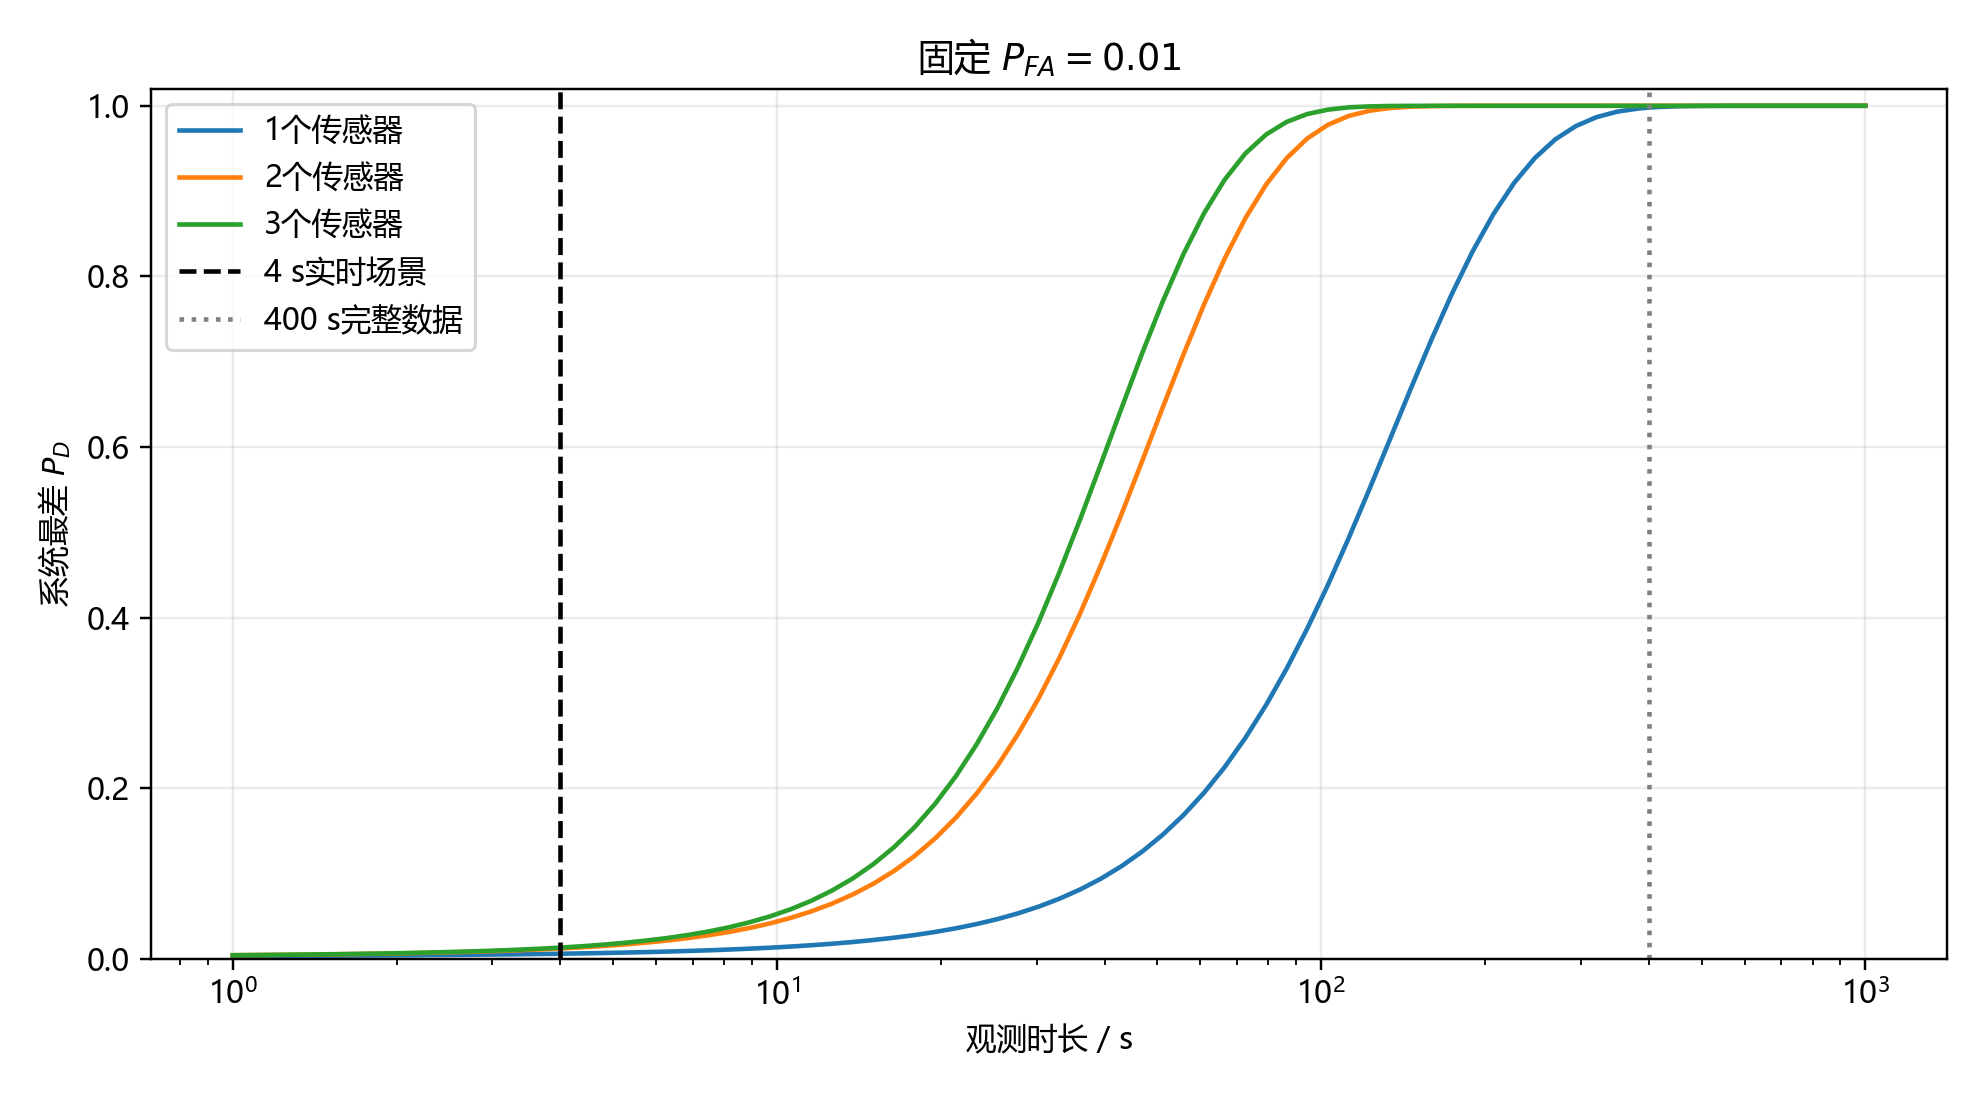
\includegraphics[width=0.88\textwidth,height=0.58\textheight,keepaspectratio]{figures/图12.png}
    \caption{积累时长对检测概率的影响}
    \label{fig:q4accum}
\end{figure}

图~\ref{fig:q4accum} 表明观测时长越长，三种方案均逐渐接近完全检测；三传感器达到 \(P_D=0.9\) 约需64.4 s，二传感器需77.8 s，单传感器需220.7 s。若工程要求数秒内报警，则需提高传感器灵敏度、降低噪声或调整系统虚警约束，不能仅靠当前布局满足。

\subsection{虚警率约束灵敏度}

进一步改变系统总虚警率约束 \(P_{FA}^{\mathrm{sys}}\)，每个水平都按式~\eqref{eq:bonferroni} 分配到四个频率，再比较不同方案的最差检测概率，结果见表~\ref{tab:pfa}。

\begin{table}[H]
\centering
\normalsize
\setlength{\tabcolsep}{4pt}
\renewcommand{\arraystretch}{1.25}
\caption{不同虚警率约束下最差故障源检测概率}
\label{tab:pfa}
\begin{tabular}{>{\centering\arraybackslash}m{3cm} >{\centering\arraybackslash}m{3cm} >{\centering\arraybackslash}m{3cm} >{\centering\arraybackslash}m{3cm}}
\toprule
系统 \(P_{FA}^{\mathrm{sys}}\) & 最优 1 传感器 \(P_D\) & 最优 2 传感器 \(P_D\) & 最优 3 传感器 \(P_D\) \\
\midrule
0.001 & 0.0008 & 0.0019 & 0.0021 \\
0.010 & 0.0060 & 0.0121 & \textbf{0.0132} \\
0.050 & 0.0243 & 0.0428 & 0.0459 \\
\bottomrule
\end{tabular}
\end{table}

\begin{figure}[H]
    \centering
    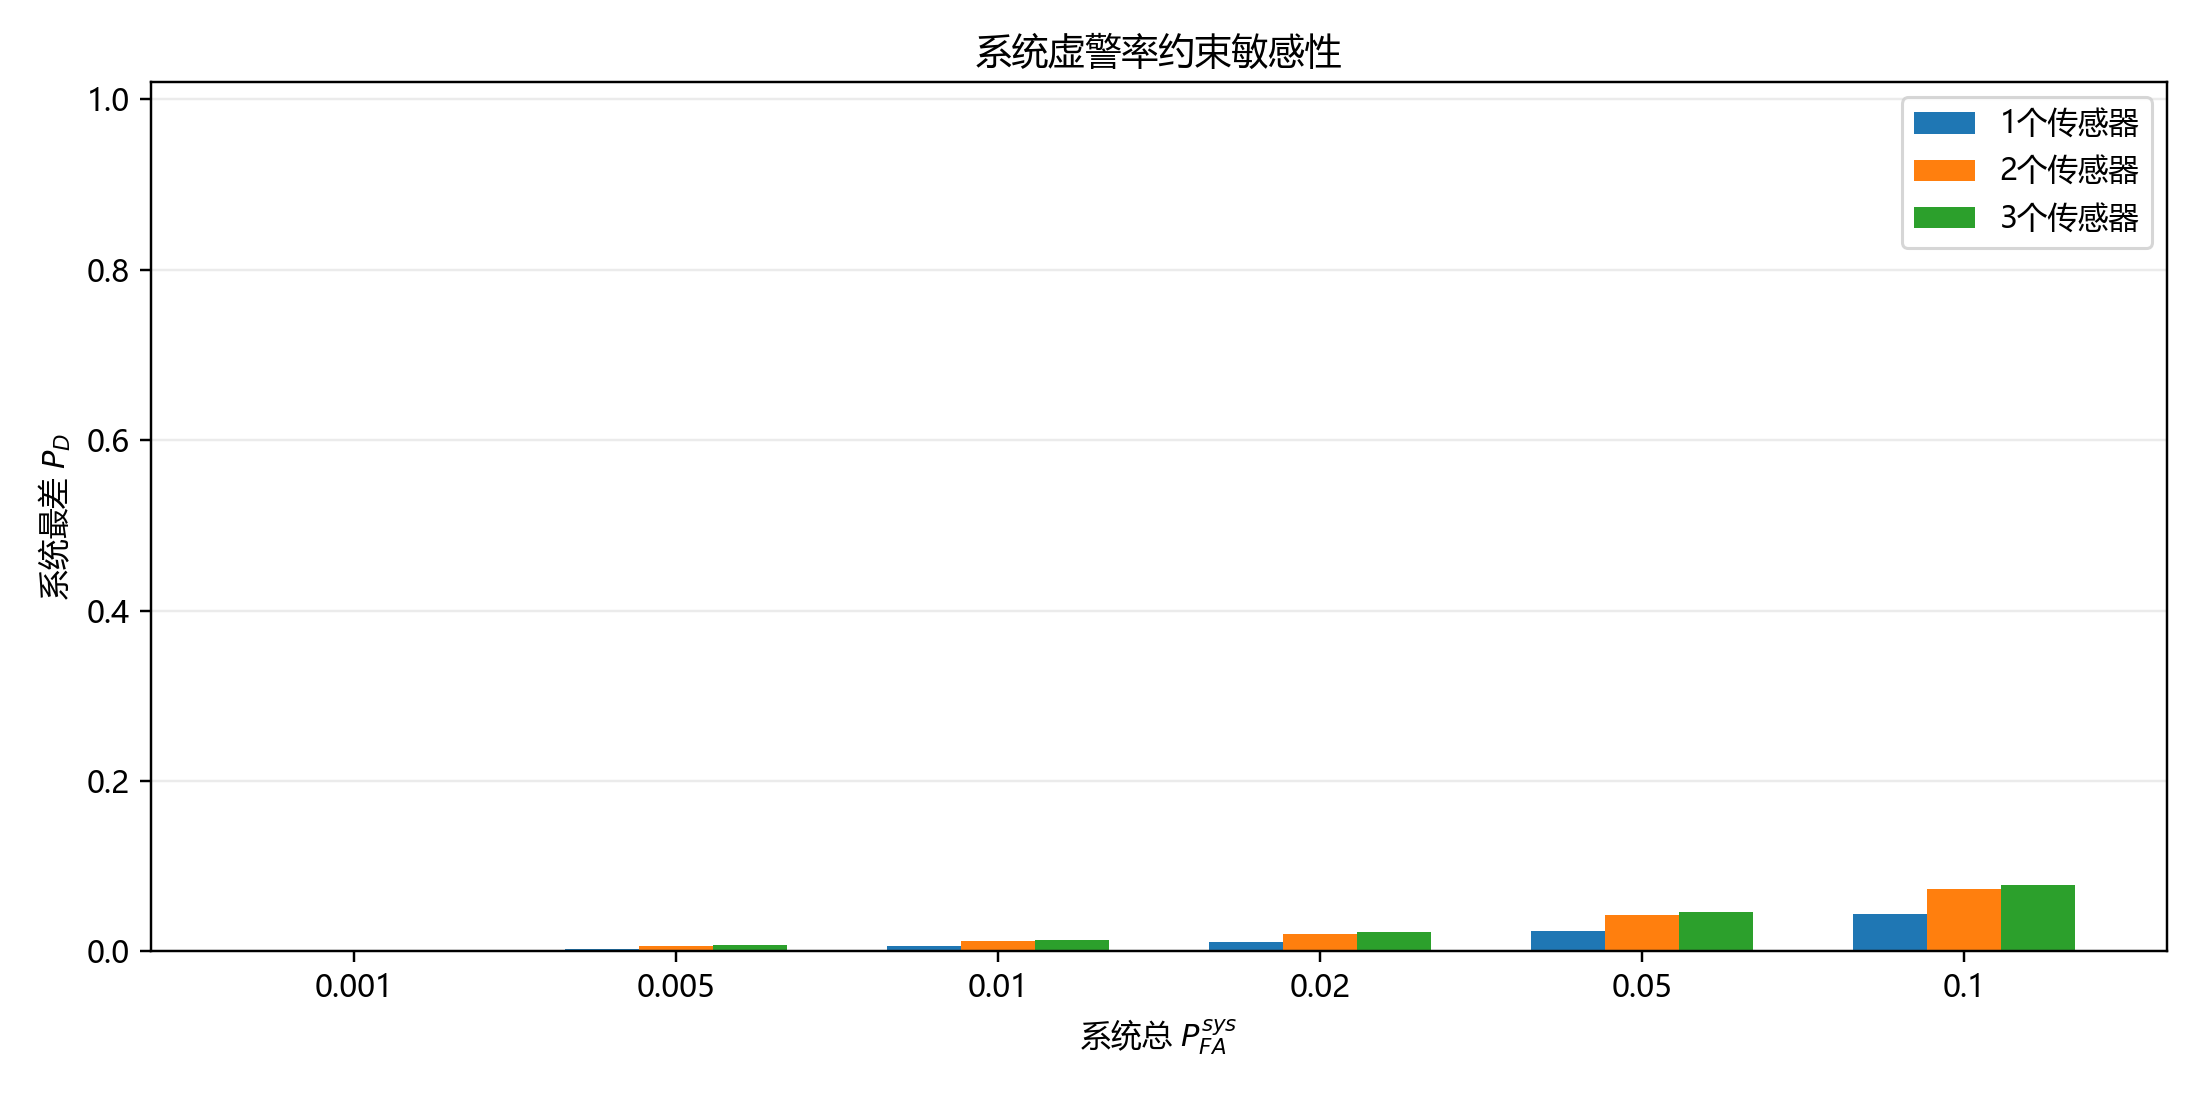
\includegraphics[width=0.88\textwidth,height=0.58\textheight,keepaspectratio]{figures/图13.png}
    \caption{虚警率约束下的检测性能}
    \label{fig:q4pfa}
\end{figure}

图~\ref{fig:q4pfa} 表明，在六个系统总虚警率水平下三传感器均优于单传感器；同时，绝对 \(P_D\) 会随 \(P_{FA}^{\mathrm{sys}}\) 明显变化。因此可靠表述应为“方案排序稳定”，而不是“检测概率对虚警率不敏感”。

\subsection{消融实验与可复现性检查}

表~\ref{tab:ablation} 从方法链条角度说明各模块的必要性；该表属于结构性分析，不替代前述数值敏感性和蒙特卡洛校准。

\begin{table}[H]
\centering
\normalsize
\setlength{\tabcolsep}{4pt}
\renewcommand{\arraystretch}{1.25}
\caption{模型关键模块消融分析}
\label{tab:ablation}
\begin{tabular}{>{\centering\arraybackslash}m{2.5cm} m{5.0cm} m{4.6cm}}
\toprule
消融项 & 去除后的影响 & 结论 \\
\midrule
去除 Welch 验证 & 仅凭单段 FFT，噪声基底起伏增大，峰值稳定性证明不足 & Welch 提供稳健性证据 \\
去除 \(\mathrm{BIC}\) 选阶 & 需要人工指定 \(M\)，容易漏检弱峰或过拟合噪声峰 & \(\mathrm{BIC}\) 使多源分离自动化 \\
去除联合 LS & 各频率分量逐个拟合会产生相互泄漏 & 联合估计能同时校正各分量 \\
去除非相干能量融合 & 传感器只能局部检测，无法提升全局最差 \(P_D\) & 融合是提升系统级性能的关键 \\
\shortstack{去除 max-min\\目标} & 可能使强源检测过好、弱源漏检 & max-min 保证最差故障源可靠性 \\
\bottomrule
\end{tabular}
\end{table}

\section{模型评价与改进}

\textbf{模型优点：}四问由检测、恢复、分离到布局递进，谱估计、正交投影、BIC、Bonferroni控制与max-min优化相互衔接；频率、振幅、区间、残差、\(P_D\) 和灵敏度均有定量结果。真实图纸、传播标定和噪声测量可直接替换算例输入，算法具有可核验性与可迁移性。

\textbf{模型不足：}非平稳冲击、转速谐波和测点相关噪声仍需现场检验；指数衰减未描述反射、多路径及局部刚度变化；恒速假设不适用于明显变速工况；候选点或传感器数量很大时，穷举计算量迅速增加。

\textbf{推广改进：}变速工况可引入阶次谱或同步重采样，未知频率检测可采用GLRT与Bootstrap；系统层面可用实测频率响应替代指数衰减，并把成本、安装可达性和冗余容错纳入多目标布局。

\section{结论}

本文对原始数据、统计量尺度和问题四题设条件进行了统一核验。单源频率为 \(2.0000\,\mathrm{Hz}\)，恢复振幅与初相为0.0352和 \(1.574\,\mathrm{rad}\)；500次有真值仿真的波形NRMSE中位数为4.47\%。多源模型由BIC选择四阶，\(\Delta\mathrm{BIC}_{5-4}=13.36\)，连续精化频率为 \(4.0000\)、\(7.9999\)、\(13.0001\)、\(14.0000\,\mathrm{Hz}\)，残差RMSE为0.0999。

问题四在系统总虚警率0.01下给出max--min三点布局：典型设备布于左右轴承座与中部齿轮箱，其他结构沿传播路径分散布于关键承载部位。代表性算例中，三传感器使达到 \(P_D=0.9\) 的时间由220.7 s降至64.4 s。

\begin{thebibliography}{99}
\bibitem{lv2022} LV Y, YANG D, YUAN R, et al. A novel multivariate signal processing-based fault diagnosis approach of rotating machinery under various operating conditions[J]. Measurement Science and Technology, 2022, 33(7): 075106. DOI: 10.1088/1361-6501/ac60d5.
\bibitem{an2022} AN H, YOUN B D, KIM H S. Optimal sensor placement considering both sensor faults under uncertainty and sensor clustering for vibration-based damage detection[J]. Structural and Multidisciplinary Optimization, 2022, 65(3): 102. DOI: 10.1007/s00158-021-03159-9.
\bibitem{hassani2023} HASSANI S, DACKERMANN U. A systematic review of optimization algorithms for structural health monitoring and optimal sensor placement[J]. Sensors, 2023, 23(6): 3293. DOI: 10.3390/s23063293.
\bibitem{xiao2025} XIAO X, LI C, HE H, et al. Rotating machinery fault diagnosis method based on multi-level fusion framework of multi-sensor information[J]. Information Fusion, 2025, 113: 102621. DOI: 10.1016/j.inffus.2024.102621.
\bibitem{deepseek2025} DeepSeek, DeepSeek-V3.1, 深度求索（DeepSeek）, 2026.06.23.
\bibitem{proakis2006} PROAKIS J G, MANOLAKIS D G. Digital Signal Processing[M]. 4th ed. Upper Saddle River: Pearson, 2007.
\bibitem{bendat2010} BENDAT J S, PIERSOL A G. Random Data: Analysis and Measurement Procedures[M]. 4th ed. Hoboken: Wiley, 2010.
\bibitem{welch1967} WELCH P D. The use of fast Fourier transform for the estimation of power spectra: A method based on time averaging over short, modified periodograms[J]. IEEE Transactions on Audio and Electroacoustics, 1967, 15(2): 70--73. DOI: 10.1109/TAU.1967.1161901.
\bibitem{kay1993} KAY S M. Fundamentals of Statistical Signal Processing, Volume I: Estimation Theory[M]. Englewood Cliffs: Prentice Hall, 1993.
\bibitem{schwarz1978} SCHWARZ G. Estimating the dimension of a model[J]. The Annals of Statistics, 1978, 6(2): 461--464. DOI: 10.1214/aos/1176344136.
\bibitem{neyman1933} NEYMAN J, PEARSON E S. On the problem of the most efficient tests of statistical hypotheses[J]. Philosophical Transactions of the Royal Society A, 1933, 231: 289--337. DOI: 10.1098/rsta.1933.0009.
\end{thebibliography}

\newpage

\section*{附录：支撑材料与完整程序}
\addcontentsline{toc}{section}{附录：支撑材料与完整程序}

\subsection*{附录 A：支撑材料清单}

根据竞赛论文格式规范，附录列出支撑论文结果的文件。原始试验代码不作为论文结果依据，也不在附录展示；表~\ref{tab:support-files} 中的最终程序是唯一用于生成本文数值、表格和图件的版本。

\begin{table}[H]
\centering
\small
\renewcommand{\arraystretch}{1.2}
\caption{支撑材料文件清单}
\label{tab:support-files}
\begin{tabular}{>{\centering\arraybackslash}m{1.0cm} m{4.6cm} m{6.6cm}}
\toprule
序号 & 文件或目录 & 说明 \\
\midrule
1 & \texttt{code/final\_analysis.py} & 最终完整程序；统一完成问题一至问题四并生成全部论文结果 \\
2 & \texttt{code/requirements.txt} & Python 依赖及经复现实验验证的版本 \\
3 & \texttt{generated/results.json} & 论文关键数值的机器可读汇总 \\
4 & \texttt{generated/tables/} & 方法比较、BIC、分辨实验、布局及灵敏度结果 \\
5 & \texttt{generated/figures/} & 由最终程序生成的图1--12 \\
\bottomrule
\end{tabular}
\end{table}

\subsection*{附录 B：运行环境与复现方法}

运行环境为 Windows 11、Python 3.13.13；主要依赖为 NumPy 2.4.4、Pandas 3.0.2、SciPy 1.17.1、Matplotlib 3.10.8 和 openpyxl 3.1.5。在论文根目录执行
\begin{lstlisting}[language=bash,basicstyle=\ttfamily\small]
python -m pip install -r code/requirements.txt
python code/final_analysis.py
\end{lstlisting}
即可读取题目附件 \texttt{A题：机械设备故障检测/data.xlsx}，并在 \texttt{generated/} 下重新生成全部输出。随机实验采用固定种子 \texttt{20260622}，以保证结果可复现。

\subsection*{附录 C：最终完整源代码}

\lstinputlisting[
  language=Python,
  basicstyle=\ttfamily\fontsize{5.5pt}{6.2pt}\selectfont,
  breaklines=true,
  breakatwhitespace=false,
  breakindent=0pt,
  columns=flexible,
  caption={问题一至问题四统一求解程序},
  label={code:final}
]{code/final_analysis.py}

\end{document}
